\documentclass[twoside,bibliography=totoc,openany]{scrbook}
%\setcounter{secnumdepth}{0}
%\usepackage{showframe}
\usepackage{amsmath,amssymb}
\numberwithin{figure}{section}
\numberwithin{table}{section}
\makeatletter
\newcommand{\mathleft}{\@fleqntrue\@mathmargin0pt}
\newcommand{\mathcenter}{\@fleqnfalse}
\makeatother
\usepackage{enumerate}
\usepackage{geometry}
\usepackage{ifoddpage}
\usepackage{calc}
\usepackage{lipsum}
\usepackage{changepage}
\usepackage{graphicx}
\usepackage{blindtext}
\usepackage[bottom]{footmisc}
\usepackage[ngerman]{babel}
\usepackage{wrapfig}
\usepackage{float}
\usepackage{titletoc}
%\restylefloat{table}
%\usepackage{sidenotes}
%\usepackage{mwe}
\usepackage[utf8]{inputenc}

%custom packages not from template
\usepackage{silence}
\WarningFilter{scrbook}{Usage of package `fancyhdr'}

\usepackage{minted}
\usepackage{microtype}
\usepackage{cleveref}
%end of custom packages not from template

\usepackage[bookmarks,hypertexnames=false,debug,hidelinks]{hyperref}
\usepackage{bookmark}
\usepackage{nameref} 
\usepackage[listformat=empty]{caption}
\captionsetup{justification=raggedright,singlelinecheck=false}
\usepackage{marginnote}
\usepackage[export]{adjustbox}
\usepackage{tocloft}
\renewcommand{\cftchapleader}{\cftdotfill{\cftdotsep}}
\renewcommand{\cftsecleader}{\cftdotfill{\cftdotsep}}
\usepackage{fancyhdr}
\usepackage{frutiger}
\usepackage{lmodern}
\setlength{\cftfignumwidth}{-15pt}
\setlength{\cfttabnumwidth}{-15pt}
\DeclareCaptionType{formel}[][Formelverzeichnis]
\captionsetup[formeln]{labelformat=empty}
\usepackage[style=numeric, citestyle=numeric, backend=biber]{biblatex}
\geometry{top=25mm, left=20mm, right=30mm, bottom=20mm}
\setlength{\marginparwidth}{10mm}

\newlength{\tempParIndent}
\newcommand{\textBody}[1]{%
    \begin{minipage}[t]{\linewidth-5cm-\marginparsep}
    \setlength{\parindent}{\tempParIndent}%
        #1
    \end{minipage}%
    }
\newcommand{\noteBody}[1]{%
    \begin{minipage}[t]{50mm}
        #1
    \end{minipage}%
}
\newcommand{\textAndNote}[2]{%
    % input:
    % #1: The main text
    % #2: The note
    \setlength{\tempParIndent}{\parindent}
    \begin{adjustwidth*}{}{-\marginparwidth-\marginparsep}%
    \checkoddpage%
\ifoddpage%
    \textBody{#1}%
    \hspace{\marginparsep}%
    \noteBody{#2}%
\else%
    \noteBody{#2}%
    \hspace{\marginparsep}%
    \textBody{#1}%
\fi%
    \end{adjustwidth*}}

\addbibresource{literatur.bib}

\begin{document}

\begin{titlepage}
    \title{Fehlersuche und Visualisierung der Belegung von
    Synchronisationsmitteln in nebenläufigen Systemen}
    \date{30. April 2020}
    \author{Marcel Sobottka}
    \publishers{
        Erstgutachter: Prof. Dr.-Ing. habil. Herwig Unger\\
        Zweitgutachter: Unbekannt\\
        Betreuer: Dipl.-Inform. (Univ.) Marcel Schaible}

    \maketitle
\end{titlepage}

\newpage\null\thispagestyle{empty}\newpage
\cleardoubleoddpage
\addtocontents{toc}{~\hfill\textbf{Seite}\endgraf}
\pagenumbering{Roman}
\setcounter{page}{3}
\tableofcontents
\thispagestyle{fancy}
% clear all header fields
\fancyhead{} 
%\fancyhead[RO,LE]{\thepage}
\fancyhead[R]{\thepage}
\fancyfoot{}
\addcontentsline{toc}{chapter}{Inhaltsverzeichnis}
\newpage \phantomsection \listoffigures
\thispagestyle{fancy}
% clear all header fields
\fancyhead{} 
%\fancyhead[RO,LE]{\thepage}
\fancyhead[R]{\thepage}
\fancyfoot{}
\addcontentsline{toc}{chapter}{Abbildungsverzeichnis}
\newpage \phantomsection \listoftables
\thispagestyle{fancy}
% clear all header fields
\fancyhead{} 
%\fancyhead[RO,LE]{\thepage}
\fancyhead[R]{\thepage}
\fancyfoot{}
\addcontentsline{toc}{chapter}{Tabellenverzeichnis}
\newpage \phantomsection
% \listofformel \thispagestyle{fancy} \fancyhead{} clear all header fields
% \fancyhead[RO,LE]{\thepage} \fancyfoot{}
% \addcontentsline{toc}{chapter}{Formelverzeichnis} \newpage
\clearpage
\pagenumbering{arabic}  
\setcounter{page}{6}
\parindent 0pt
\fancypagestyle{plain}{%
\fancyhf{}\renewcommand{\headrulewidth}{0pt}}
\pagestyle{fancy}
\renewcommand{\chaptermark}[1]{\markboth{#1}{}}
\renewcommand{\sectionmark}[1]%
{\markboth{#1}{}}
\fancyhead{} % clear all header fields
%\fancyhead[RE,LO]{\leftmark}
%\fancyhead[RO,LE]{\thepage}
\fancyhead[L]{\leftmark}
\fancyhead[R]{\thepage}
\fancyfoot{}

\startcontents
\chapter{Motivation}
\thispagestyle{fancy}
Bei der parallelen Entwicklung werden nebenläufige Anwendungen erstellt, in
denen Aufgaben definiert werden, deren Ausführungsreihenfolge nicht festgelegt
ist. Die Ausführung von nebenläufigen Programmen ist nicht deterministisch.
Mehrere parallele Aufgaben können bei jeder Ausführung eines solchen Programms
in einer anderen Reihenfolge abgearbeitet werden. Dies führt dazu, dass Zugriffe
auf gemeinsam genutzte Ressourcen synchronisiert werden müssen.

Bei der Synchronisierung können zur Laufzeit sogenannte Deadlocks (engl.
Verklemmungen) auftreten. Für Entwickler stellen Deadlocks ein großes Problem
dar, da sie oft erst zur Laufzeit auffallen. Während der Entwicklung kann ein
Entwickler Nebenläufigkeitsprobleme, die zu Deadlocks führen können, nur sehr
schwer erkennen. Gerade in komplexen Anwendungen, in denen viele parallele
Aufgaben ausgeführt werden, ist es für den Entwickler nicht mehr möglich,
potenzielle Deadlocks zu erkennen. Durch automatisierte Tests können solche
Probleme zwar teilweise nachgewiesen werden, durch die nicht deterministische
Ausführung bleiben jedoch viele Probleme unerkannt. Für die
Echtzeit-Programmiersprache PEARL gibt es derzeit keine Unterstützung für den
Entwickler, um solche Probleme effektiv zu erkennen. Um den Entwickler besser
unterstützen zu können, soll in dieser Arbeit ein Verfahren vorgestellt und
implementiert werden, welches die chronologische Abfolge von verwendeten
Synchronisationsmitteln darstellen und potenzielle Deadlocks erkennen kann. Das
Ziel dieser Arbeit besteht darin Entwicklern eine einfache Möglichkeit zu bieten
potentielle Deadlocks in PEARL-Programmen zu finden.

In \cref{section:Deadlock-Erkennung allgemein} wird das grundlegende Verfahren
zur Identifizierung von potenziellen Deadlocks vorgestellt. Es wird beschrieben,
was ein Deadlock ist und wie dynamische Verfahren zur Erkennung von Deadlocks
funktionieren. In \cref{section:PEARL} wird die Echtzeit-Programmiersprache
PEARL beschrieben. Es wird gezeigt, welche Synchronisationsmittel in PEARL
existieren und wie diese benutzt werden. Anschließend wird in
\cref{section:OpenPEARL} das OpenPEARL Projekt, der Aufbau der
OpenPearl-Umgebung und das Zusammenspiel des Compilers und der Laufzeitumgebung
dargestellt. In \cref{section:MagicLock} wird ein Algorithmus zur Erkennung von
potenziellen Deadlocks vorgestellt. Anhand eines Quellcode-Beispiels in PEARL
wird der Algorithmus Schritt für Schritt durchlaufen und erläutert. 

Das Design zur Implementierung des Algorithmus wird in \cref{chapter:Design}
beschrieben. In \cref{section:Analysieren der Trace-Datei} wird der in OpenPEARL
umzusetzende Anteil definiert um die benötigten Informationen für den
Algorithmus in einer Trace-Datei zusammenzustellen. In \cref{section:Analysieren
der Trace-Datei} und \cref{section:Erweiterung: Potenzielle Deadlocks} werden
die Designs der Programmme zur Visualisierung der chronologischen Belegung der
Synchronisationsmittel und der Erkennung von potenziellen Deadlocks definiert.

In \cref{section:Implementierung:Trace-Funktion} wird die Implementierung zur
Erstellung der Trace-Datei in OpenPEARL beschrieben. Anschließend werden die
Implementierungen der Programmme zur Analyse und Visualisierung der Trace-Datei
in \cref{section:Implementierung:Analyse-Programm} und
\cref{section:Implementierung:Visualisierung von potenziellen Deadlocks}
vorgestellt.

Die Validierung der in \cref{chapter:Implementierung} erstellten Programme und
Funktionen wird in \cref{chapter:Validierung} durchgeführt.

Abschließend werden in \cref{chapter:Ausblick} die Ergebnisse der Arbeit
zusammengefasst und offene Punkte und mögliche Weiterentwicklungen beschrieben. 
\stopcontents

\startcontents
\chapter{Analyse}
\thispagestyle{fancy}
\printcontents{l}{1}{\setcounter{tocdepth}{5}}
\section{Deadlockerkennung allgemein}
\label{section:Deadlockerkennung allgemein}
Üblicherweise gliedern sich Programme in  Single-Threaded- und
Multi-Threaded-Anwendungen, das heißt Anwendungen die entweder nur von einem
Thread ausgeführt werden oder von mehreren gleichzeitig. Im Gegensatz zu
Single-Threaded-Anwendungen sind Multi-Threaded-Anwendungen nicht
deterministisch. Dies kann zu sogenannten \emph{race conditions} (engl.
Wettlauf-Bedingung) führen. Eine \emph{race condition} tritt zum Beispiel dann
auf, wenn zwei Threads einen Zähler jeweils um 1 erhöhen wollen\footnote{Vgl.
"`Data races"' in \autocite[70]{netzer1992race}}.

Ein einfaches Beispiel: Angenommen der Zähler hat zu Beginn den Wert 3. Beide
Threads wollen jetzt nahezu gleichzeitig den Zähler um 1 erhöhen. Dazu lesen
beide Threads den aktuellen Wert des Zählers, in diesem Fall 3, aus.
Anschließend addieren beide den Wert 1 hinzu und schreiben den neuen Wert, in
diesem Fall 4, in den Zähler. Erwartet wurde jedoch der Wert 5, da beide Threads
den Zähler um jeweils 1 erhöhen sollten. Um solche \emph{race conditions} zu
verhindert werden Synchronisationsmechanismen benötigt.

Eine Möglichkeit um den Zugriff auf eine gemeinsame Ressource zu
synchronisieren, sind sogenannte Locks. Ein Lock ist ein exklusiver Zugriff auf
ein Objekt, ein sogenanntes Lockobjekt. Das bedeutet, dass während ein Thread
einen Lock auf ein Objekt besitzt, andere Threads, welche auf dasselbe Objekt
zugreifen wollen, warten müssen, bis es freigegeben wurde.

Betrachtet man das Beispiel mit dem Zähler erneut, dieses Mal mit Locks als
Synchronisationsmittel, kann es zu folgender Ausführung kommen. Der Zähler hat
zu Beginn wieder den Wert 3. Die Threads \textrm{T1} und \textrm{T2} wollen
erneut den Zähler nahezu gleichzeitig erhöhen. Dieses Mal versuchen beide das
Lockobjekt \textrm{L1} in Besitz zu nehmen. Der Thread \textrm{T2} nimmt
\textrm{L1} zuerst in Besitz, daraus folgt, dass \textrm{T1} muss warten. \textrm{T2}
liest den aktuellen Wert des Zählers aus, erhöht diesen um 1 und schreibt den
neuen Wert 4 in den Zähler. Anschließend gibt \textrm{T2} das Lockobjekt
\textrm{L1} frei. Jetzt erhält der Thread \textrm{T1} den Zugriff auf
\textrm{L1} und liest ebenfalls den Zähler, jetzt 4, aus, erhöht diesen und
schreibt den neuen Wert 5 in den Zähler. Anschließend gibt \textrm{T1} das
Lockobjekt \textrm{L1} frei. Jetzt steht der erwartete Wert 5 im Zähler. Durch
das Lockobjekt ist die Ausführung weiterhin nicht deterministisch, da die
Reihenfolge auch erst \textrm{T1} und dann \textrm{T2} sein kann. Trotzdem ist
die korrekte Erhöhung des Zählers sichergestellt.

Die Verwendung von Locks kann in Verbindung mit der nicht deterministischen
Ausführung von Multi-Threaded-Anwendungen zu Problemen führen.

Angenommen, es existieren zwei Threads \textrm{T1} und \textrm{T2} und zwei
Lockobjekte \textrm{L1} und \textrm{L2}. Angenommen, \textrm{T1} besitzt
\textrm{L1} und zur gleichen Zeit erlangt \textrm{T2} das Lockobjekt
\textrm{L2}. Wenn jetzt der Thread \textrm{T1} das Lockobjekt \textrm{L2}
anfordert und der Thread \textrm{T2} das Lockobjekt \textrm{L1}, kommt es zu
einem Deadlock.\autocite[vgl.][70]{coffman1971system} Die Ausführung des
Programms terminiert nicht, da beide Threads auf den jeweils anderen Thread
warten und sich gegenseitig blockieren.

Solche potenziellen Deadlocks zu erkennen, ist die Aufgabe von statischen und
dynamischen Methoden zur Deadlockerkennung. Bei der statischen Deadlockerkennung
wird der Quellcode direkt analysiert. Dieses Verfahren wird hier nicht näher
betrachtet.

Bei der dynamischen Deadlockerkennung wird die Anwendung zur Laufzeit analysiert
und läuft in folgenden drei Schritten ab
\autocite[vgl.][212-213]{bensalem2005dynamic}:
\begin{enumerate}
  \item Erstellung eines \emph{execution traces},
  \item Erstellung eines Graphen basierend auf den Informationen aus dem
  \emph{execution trace},
  \item Suche nach potenziellen Deadlocks durch die Identifizierung von Zyklen
  innerhalb des Graphen.
\end{enumerate}
Ein \emph{execution trace} ist eine Abfolge von Events. Ein Event \textrm{$e_i$}
wird durch eine der folgenden Methoden definiert: Starten eines Threads,
Betreten eines Threads, Inbesitznahme eines Lockobjekts und Freigabe eines
Lockobjekts \autocite[vgl.][212]{bensalem2005dynamic}.

Ein Event im \emph{execution trace} enthält immer auch eine Positionsangabe in
Form einer Zeilennummer \autocite[vgl.][212]{bensalem2005dynamic}. Diese
Positionsangabe  wird hier ignoriert, da sie nicht benötigt wird.\footnote{Vgl.
"`line number lno"' in \autocite[212]{bensalem2005dynamic}}

Das Starten eines neues Threads ist definiert durch ein Thread-Start-Event:
\begin{quote}
\texttt{s(ausführender Thread, Name des neuen Threads)}
\end{quote}
Zum Beispiel bedeutet \texttt{s(main,T1)}, dass der Thread \textrm{main} den
Thread \textrm{T1} gestartet hat. Das Betreten eines Threads ist definiert durch
ein Thread-Join-Event:
\begin{quote}
\texttt{j(ausführender Thread, Name des zu betretenden Threads)}
\end{quote}
Zum Beispiel bedeutet \texttt{j(T1,T2)}, dass der Thread \textrm{T1} den Thread
\textrm{T2} betreten hat. Die Inbesitznahme eines Lockobjekts kann definiert
werden durch ein Lock-Event:
\begin{quote}
\texttt{l(ausführender Thread, Name des Lockobjekts)}
\end{quote}
Zum Beispiel bedeutet \texttt{l(T1,L3)}, dass der Thread \textrm{T1} das
Lockobjekt \textrm{L3} in Besitz genommen hat. Die Freigabe eines Lockobjekts
kann definiert werden durch ein Unlock-Event:
\begin{quote}
\texttt{u(ausführender Thread, Name des Lockobjekts)}
\end{quote}
Zum Beispiel bedeutet \texttt{u(T1,L3)}, dass der Thread \textrm{T1} das
Lockobjekt \textrm{L3} freigegeben hat.

Die Abfolge aller während der Laufzeit des Programms aufgetretenen Events
definiert einen möglichen \emph{execution trace} des Programms. Programme,
welche mit mehreren Threads arbeiten, liefern keine deterministische Abfolge.
Jede Ausführung eines solchen Programms kann zu unterschiedlichen
\emph{execution traces} führen. 

Im zweiten Schritt wird aus dem vorher erzeugten \emph{execution trace} ein
Lockgraph erstellt.

\begin{samepage}
  Ein Lockgraph ist definiert durch:
  \begin{quote}
  \textrm{LG = (L,R)}
  \end{quote}
\end{samepage}
\textrm{L} ist die Menge aller Lockobjekte im \emph{execution trace} und \textrm{R}
die Menge aller Lockpaare. Ein Lockpaar ist definiert durch das Tupel
\textrm{(L1, L2)} für das gilt: Es existiert ein Thread, welcher das Lockobjekt
\textrm{L1} besitzt, während er einen Lock auf \textrm{L2}
anfordert.\cites[vgl.][72]{coffman1971system}[213]{bensalem2005dynamic}

Im letzten Schritt wird der erstellte Lockgraph nach potenziellen Deadlocks
durchsucht. Ein potenzieller Deadlock repräsentiert einen Zyklus im Lockgraphen
\cites[vgl.][72]{coffman1971system}. Für die Zyklensuche im Lockgraphen gibt es
verschiedene Algorithmen. Einer davon wird in \cref{section:MagicLock}
beschrieben.

\section{PEARL}
\label{section:PEARL}
Die Programmiersprache PEARL wurde in den 1970er Jahren vom Institut für
Regelungstechnik der Universität Hannover entwickelt. PEARL ist eine Abkürzung
und steht für "`Process and Experiment Automation Realtime Language"'. Die
Programmiersprache erlaubt eine komfortable, sichere und weitgehend
rechnerunabhängige Programmierung von Multitasking- und Echtzeit-Aufgaben
\autocite{PEARLHistory}. Das Deutsche Institut für Normung standardisierte PEARL
mehrmals, unter anderem 1998 in der DIN 66253-2 als PEARL90
\autocite{DIN-66253-2:1998-04} und zuletzt 2018 als SafePEARL
\autocite{DIN-66253:2018-03}. Nachfolgend werden PEARL und PEARL90 synonym
verwendet.

In PEARL bezeichnet ein \textrm{TASK} eine Aufgabe und wird entweder direkt beim
Start des Programms oder durch Signale von anderen Aufgaben gestartet.
\textrm{TASKs} werden parallel und gemäß ihrer Priorität ausgeführt
\autocite[vgl.][104]{PEARL}. Um mehrere \textrm{TASKs} zu synchronisieren gibt
es zwei Möglichkeiten: \textrm{SEMA}- und \textrm{BOLT}-Variablen
\autocite[vgl.][120]{PEARL}.

Eine \textrm{SEMA}-Variable ist ein Semaphor und dient als
Synchronisationsmittel. Sie kann als Wert nicht negative ganze Zahlen besitzen,
wobei null den Zustand "`gesperrt"' und positive Zahlen den Zustand "`frei"'
bedeuten \autocite[vgl.][120]{PEARL}. Eine \textrm{SEMA}-Variable hat zu Beginn
den Wert null. Mit dem Befehl \textrm{RELEASE} wird eine \textrm{SEMA}-Variable
um den Wert eins erhöht und erhält den Zustand "`frei"'. Mit dem
\textrm{REQUEST}-Befehl wird der Wert einer \textrm{SEMA}-Variablen um eins
verringert. Ist der Wert einer \textrm{SEMA}-Variablen null wird der ausführende
\textrm{TASK} angehalten und in eine Warteschlange eingereiht. Sobald die
Variable über den Befehl \textrm{RELEASE} wieder freigeben wird, wird der
nächste \textrm{TASK} in der Warteschlange gemäß seiner Priorität fortgeführt
\autocite[vgl.][120-121]{PEARL}. Das Zustandsdiagramm zur \textrm{SEMA}-Variable
ist in \cref{fig:SEMA_StateDiagram} dargestellt.
\begin{figure}[ht]
  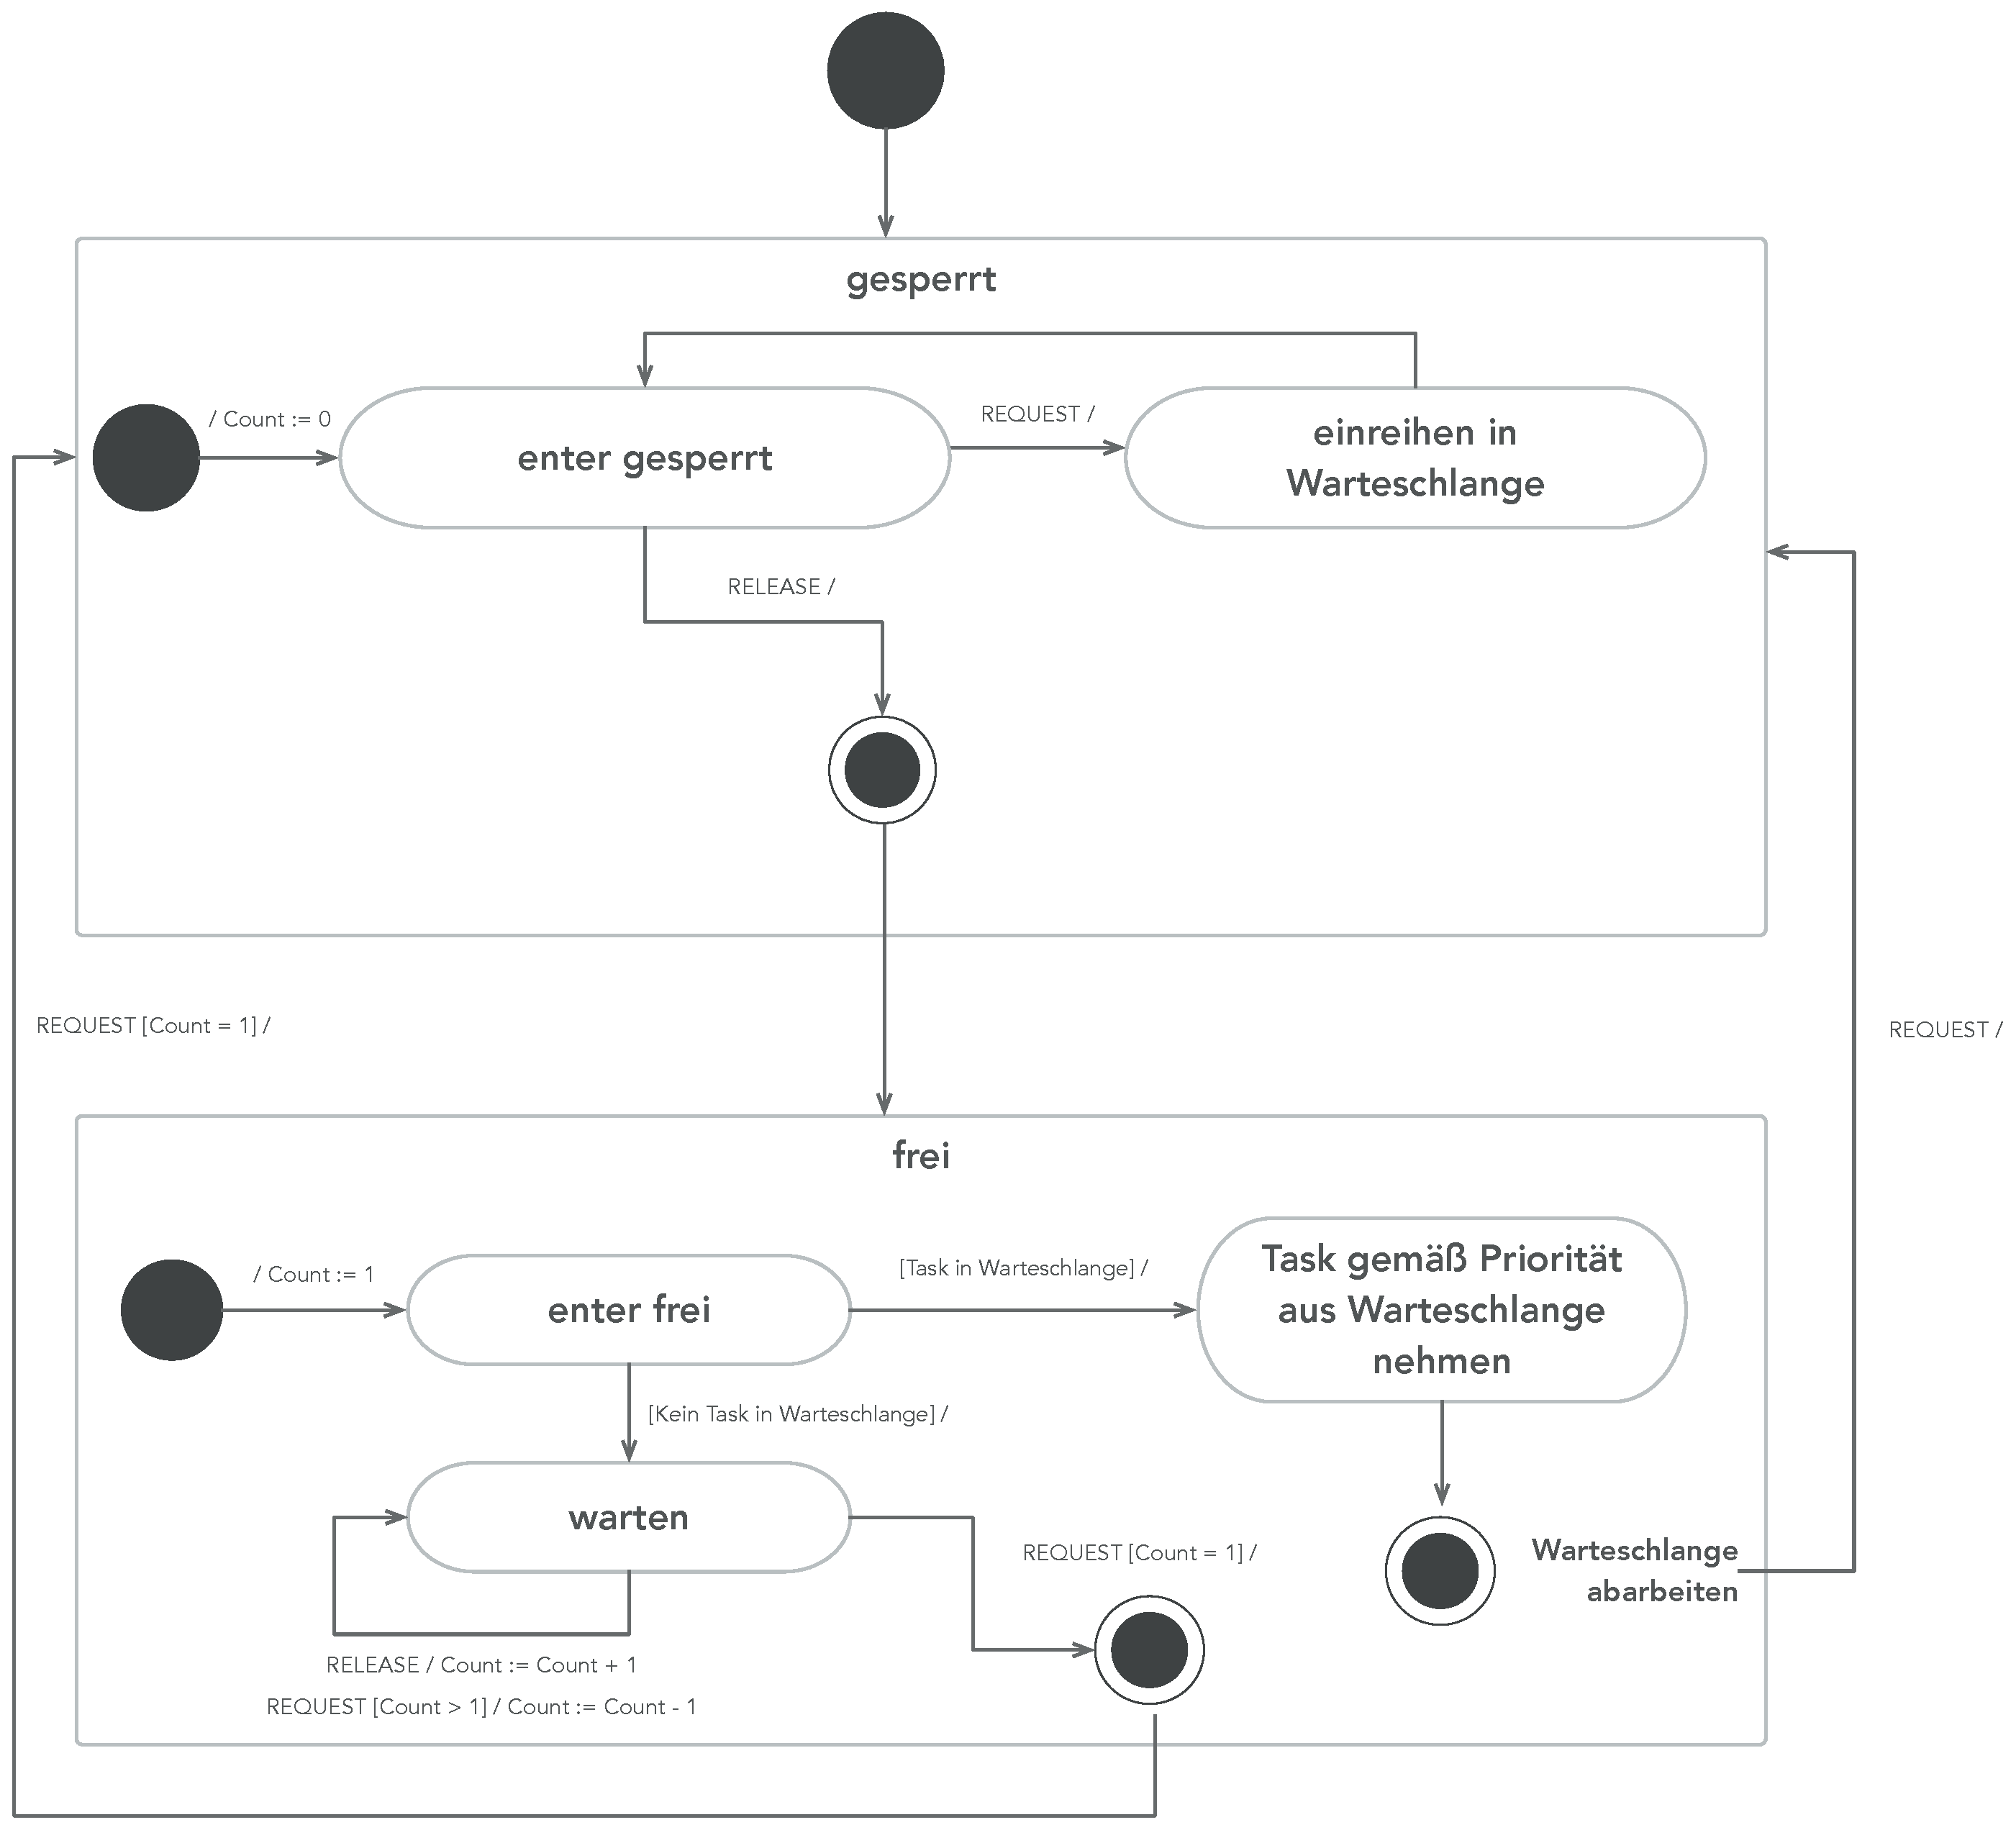
\includegraphics[width=\linewidth]{SEMA_State_Diagram.eps}
  \footnotesize\sffamily Quelle: Eigene Darstellung
  \caption{Zustandsdiagramm einer SEMA-Variablen}
  \label{fig:SEMA_StateDiagram}
\end{figure}

\textrm{BOLT}-Variablen haben im Gegensatz zu \textrm{SEMA}-Variablen drei
Zustände: "`gesperrt"', "`Sperre möglich"' und "`Sperre nicht möglich"'
\autocite[vgl.][125]{PEARL}. Sie bieten die Möglichkeit für exklusive und nicht
exklusive Sperren. Zum Beispiel können so simultane Lesezugriffe und exklusive
Schreibzugriffe realisiert werden. Zu Beginn hat eine
\textrm{BOLT}-Variable den Zustand "`Sperre möglich"'. Mit dem Befehl \textrm{RESERVE}
wird ein exklusiver Zugriff auf eine \textrm{BOLT}-Variable angefordert. Wenn
die Variable im Zustand "`Sperre möglich"' ist, erhält diese den Zustand
"`gesperrt"'. Ansonsten wird ähnlich zu der \textrm{REQUEST}-Anweisung für
\textrm{SEMA}-Variablen der ausführende \textrm{TASK} angehalten und in eine
Warteschlange eingereiht. Mit dem Befehl \textrm{FREE} erhält eine
\textrm{BOLT}-Variable den Zustand "`Sperre möglich"' und alle \textrm{TASKs} in
der Warteschlange, welche aufgrund einer \textrm{RESERVE}-Anweisung warten,
werden gemäß ihrer Priorität fortgeführt. Wenn keine \textrm{TASKs} in der
Warteschlange vorhanden sind, welche auf eine \textrm{RESERVE}-Anweisung warten,
werden die \textrm{TASKs} in der Warteschlange gemäß ihrer Priorität
fortgeführt, welche aufgrund einer \textrm{ENTER}-Anweisung warten. Mit der
\textrm{ENTER}-Anweisung wird ein nicht exklusiver Zugriff angefordert. Wenn die
\textrm{BOLT}-Variable im Zustand "`gesperrt"' ist oder ein \textrm{TASK} in der
Warteschlange existiert, welcher einen exklusiven Zugriff mittels einer
\textrm{RESERVE}-Anweisung angefordert hat, wird der ausführende \textrm{TASK}
angehalten und in eine Warteschlange eingereiht. Ansonsten erhält die Variable
den Zustand "`Sperre nicht möglich"', um den exklusiven Zugriff zu verbieten.
Zusätzlich wird die Anzahl der benutzenden \textrm{TASKs} um eins erhöht. Die
\textrm{LEAVE}-Anweisung verringert die Anzahl der benutzenden \textrm{TASKs} um
eins. Wenn die Anzahl eins entspricht, funktioniert die \textrm{LEAVE}-Anweisung
wie die \textrm{FREE}-Anweisung \autocite[vgl.][125-127]{PEARL}. Das
Zustandsdiagramm zur \textrm{BOLT}-Variable ist in \cref{fig:BOLT_StateDiagram}
dargestellt.
\begin{figure}[ht]
  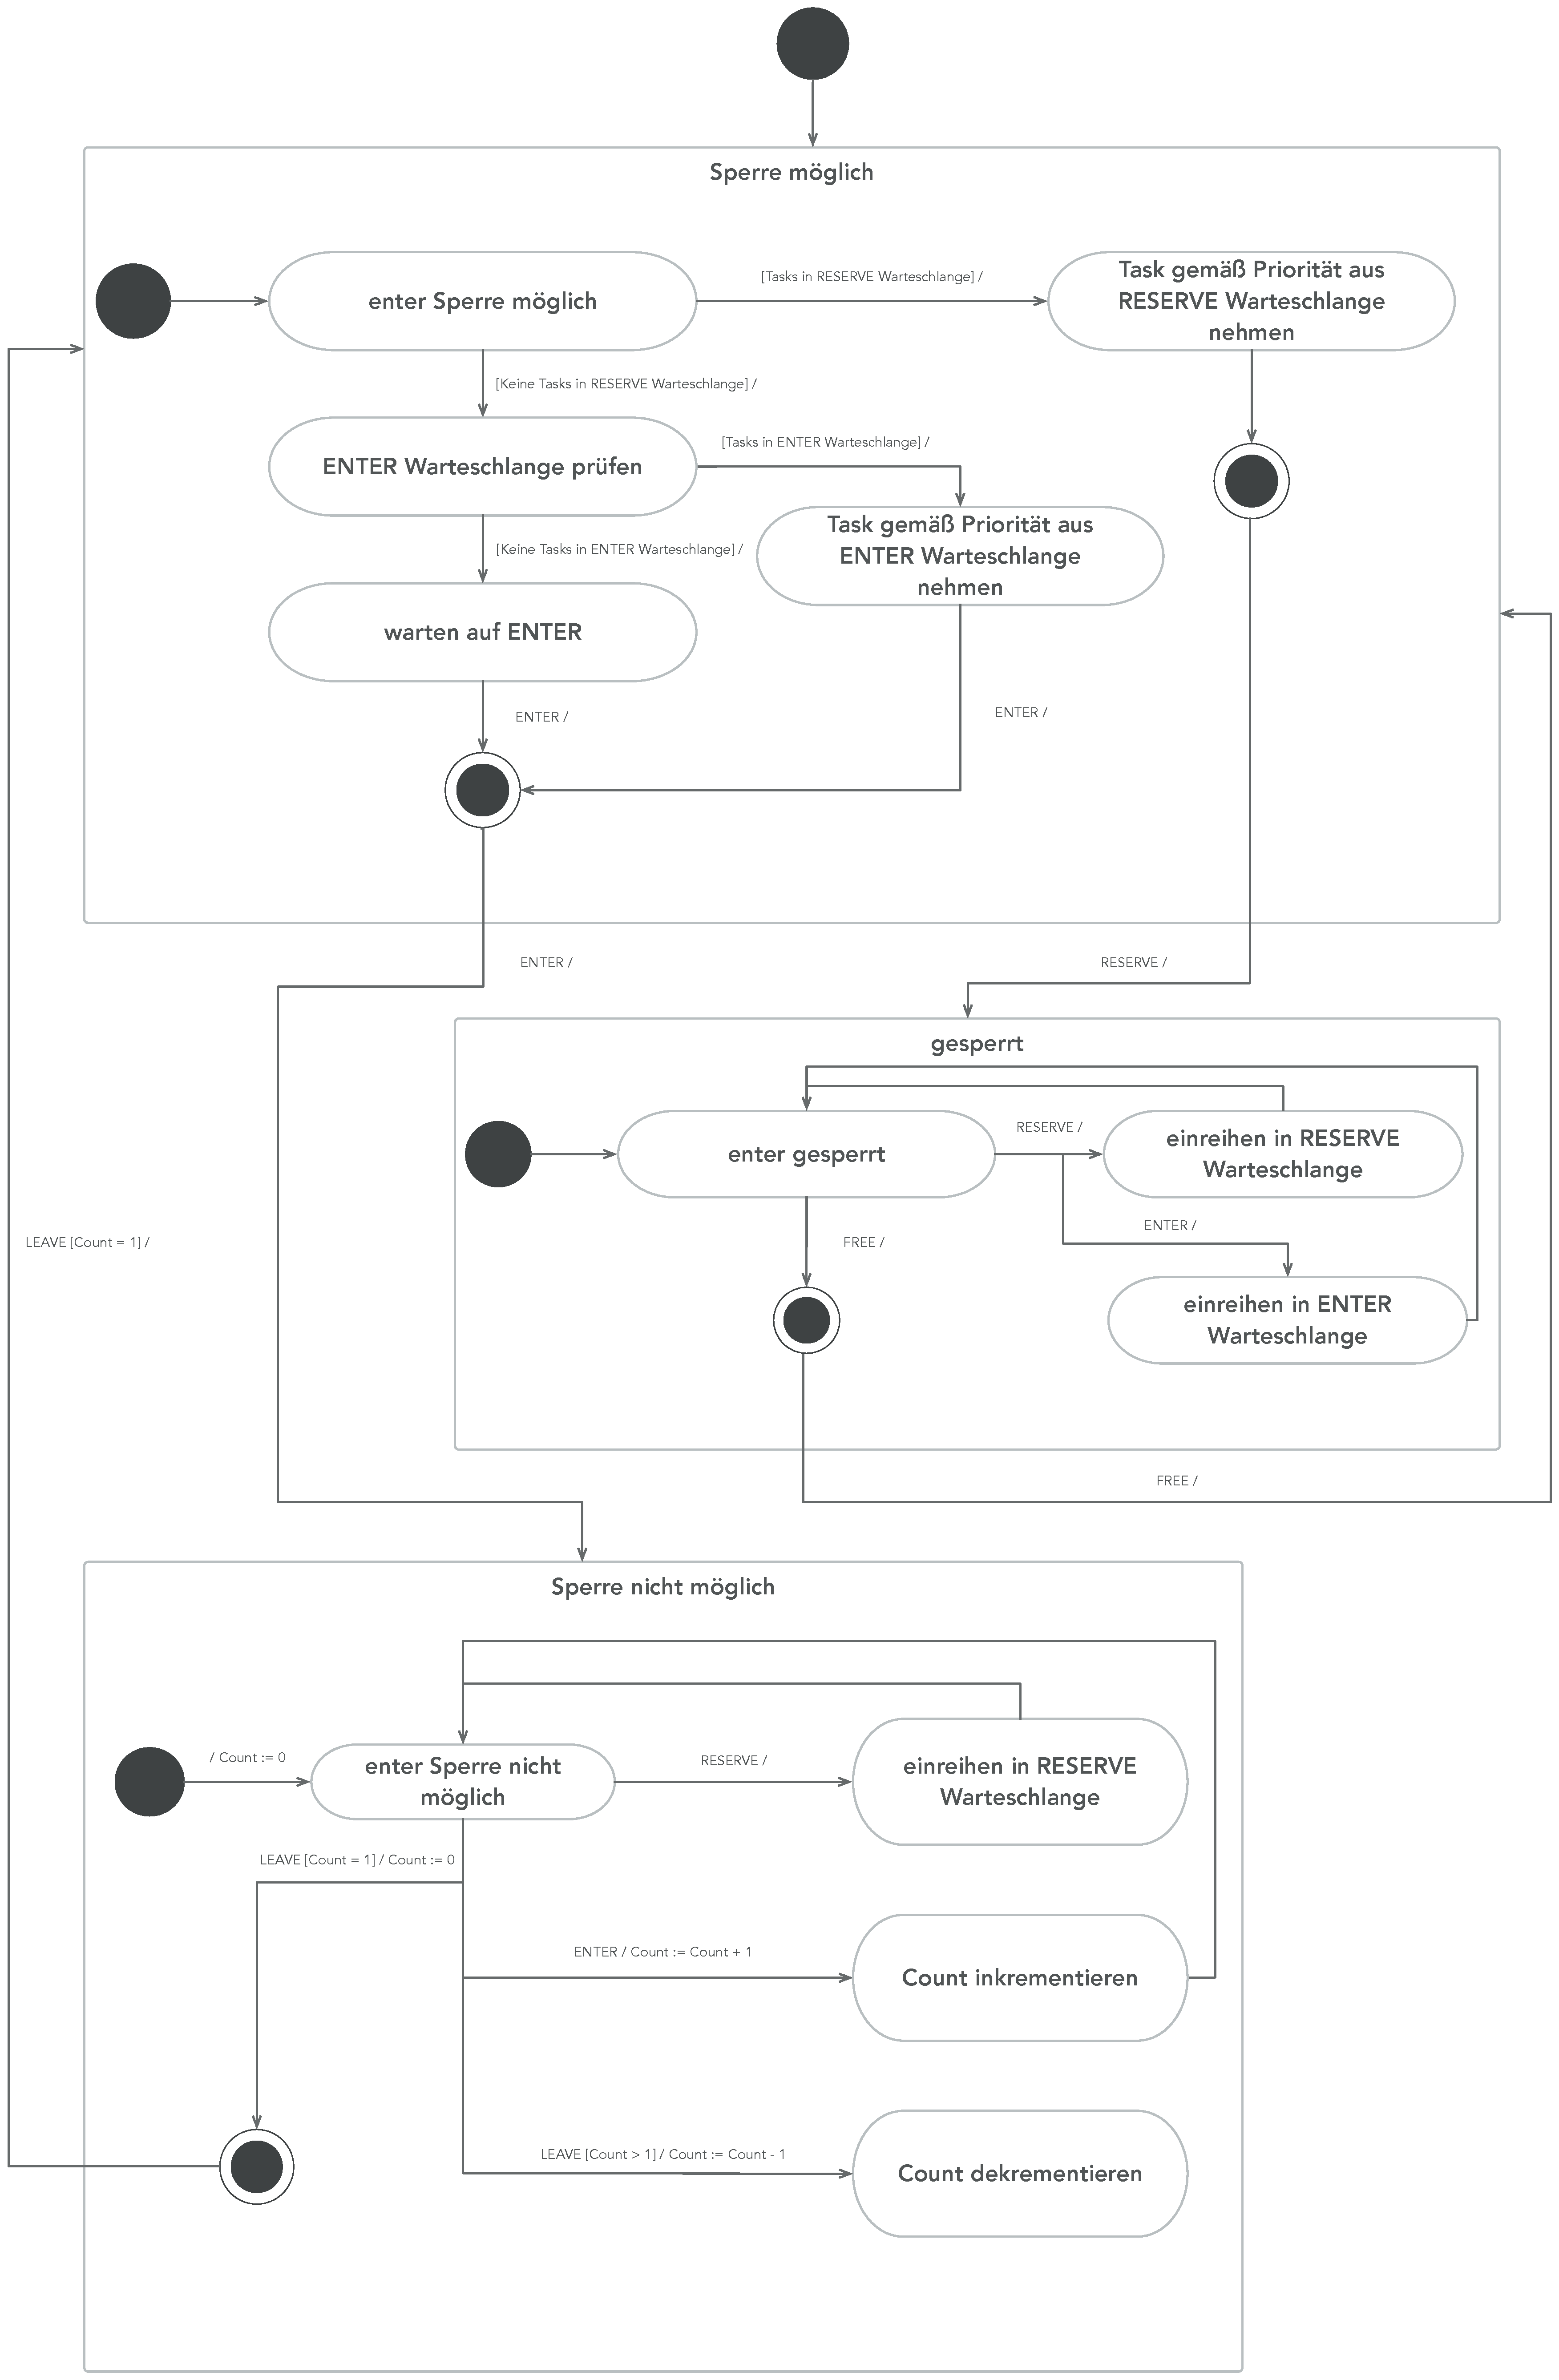
\includegraphics[width=\linewidth]{BOLT_State_Diagram.eps}
  \footnotesize\sffamily Quelle: Eigene Darstellung
  \caption{Zustandsdiagramm einer BOLT-Variablen}
  \label{fig:BOLT_StateDiagram}
\end{figure}

\section{OpenPEARL}
\label{section:OpenPEARL}
Um PEARL-Programme auf einem System auszuführen, wird ein Compiler benötigt. Das
OpenSource Projekt OpenPEARL besteht aus einem Compiler und einer
Laufzeitumgebung für PEARL \autocite{OpenPEARL_Structure}. Unterstützt wird der
PEARL90-Standard bis auf einige wenige Unterschiede
\autocite{OpenPEARL_Differences_To_PEARL90}.

OpenPEARL besteht aus drei wesentlichen Komponenten
\autocite{OpenPEARL_Structure}:
\begin{enumerate}
  \item Compiler,
  \item Laufzeitumgebung,
  \item Inter Module Checker.
\end{enumerate}
Der Compiler ist in Java geschrieben und übersetzt PEARL-Code in C++-Code. Die
Laufzeitumgebung stellt dem Compiler eine API zur Verfügung. Dem Compiler werden
durch die API sichere Implementierungen der PEARL-Datentypen zur Verfügung
gestellt. Zusätzlich enthält die Laufzeitumgebung plattformspezifische Anteile
für zum Beispiel die Implementierung für das Scheduling der Tasks.
PEARL-Anwendungen können aus mehreren Modulen bestehen, welche unabhängig
voneinander kompiliert werden. Um Inkonsistenzen bei der Erstellung der
Anwendung zu verhindern, prüft der Inter Module Checker die Export- und
Importschnittstellen aller Module und deren Kompatibilität
\autocite{OpenPEARL_Structure}.

In \cref{lst:ExampleDeadlock} ist ein Beispielprogramm in der Programmiersprache
PEARL dargestellt. Das Programm startet zwei parallele Aufgaben, welche beide
eine Zeichenfolge auf der Standardausgabe ausgeben. Der Zugriff auf die
Standardausgabe muss dabei synchronisiert erfolgen.
\begin{listing}[ht]
  \inputminted[frame=lines,linenos]{vim}{./Examples/Example_Deadlock.prl}
  \caption{Beispiel einer OpenPEARL-Anwendung mit einem potenziellen Deadlock}
  \label{lst:ExampleDeadlock}   
\end{listing} 
In den Zeilen~7 bis 10 werden Variablen definiert, wie zum Beispiel die Ausgabe
über die Standardausgabe und die zwei \textrm{SEMA}-Variablen \textrm{L1} und
\textrm{L2} in den Zeilen~9 und 10. In den Zeilen~12 bis 17 ist ein \textrm{TASK}
definiert.

Durch die Kennzeichnung \textrm{MAIN} wird der \textrm{TASK} direkt beim Start
des Programms ausgeführt \autocite[vgl.][28]{PEARL}. Die Befehle
\textrm{RELEASE} in den Zeilen~13 und 14 erhöhen den Wert der jeweiligen
\textrm{SEMA}-Variable um eins, wodurch der Zustand von "`gesperrt"' auf
"`frei"' gesetzt wird. Anschließend werden in den Zeilen~15 und 16 die
\textrm{TASKS} \textrm{T2} und \textrm{T3} gestartet.

Die \textrm{TASKS} \textrm{T2} und \textrm{T3} geben in den Zeilen~22 bis 24 und
in den Zeilen~32 bis 34 die Zeichenfolge "`Hello World T2"' bzw. "`Hello World
T3"' auf der Standardausgabe aus. Die Synchronisierung des Zugriffs auf die
Standardausgabe erfolgt mittels der \textrm{SEMA}-Variablen \textrm{L1} und
\textrm{L2}. Beide \textrm{TASKS} versuchen beide \textrm{SEMA}-Variablen in
Besitz zu nehmen. \textrm{T2} versucht in den Zeilen~20 und 21 zuerst
\textrm{L1} und dann \textrm{L2} in Besitz zu nehmen. \textrm{T3} versucht in
den Zeilen~30 und 31 zuerst \textrm{L2} und dann \textrm{L1} in Besitz zu
nehmen. Da beide \textrm{TASKS} parallel laufen, kann es passieren, dass
\textrm{T2} \textrm{L1} in Zeile~20 in Besitz nimmt und gleichzeitig \textrm{T3}
in Zeile~30 \textrm{L2} in Besitz nimmt. Beide \textrm{SEMA}-Variablen haben
jetzt den Wert null und den Zustand "`gesperrt"'. Der \textrm{TASK} \textrm{T2}
wartet jetzt darauf, dass \textrm{L2} freigegeben wird und
\textrm{T3} wartet darauf, dass \textrm{L1} freigegeben wird. Beide \textrm{TASKS}
warten auf den jeweils anderen und verursachen einen Deadlock.

\section{MagicLock}
\label{section:MagicLock}
MagicLock ist ein Algorithmus zur dynamischen Deadlockerkennung. Während der
Entwicklung wurde der Fokus auf die Skalierung und Effizienz des Algorithmus
gesetzt. Ziel war es, mit großen Multithreaded-Anwendungen skalieren und diese
effizient analysieren zu können \autocite[vgl.][1]{MagicLock}.

MagicLock analysiert einen \emph{execution trace} einer Programmausführung ohne
Deadlocks \autocite[vgl.][4]{MagicLock}. Ein möglicher \emph{execution trace}
von dem Beispielprogramm aus \cref{lst:ExampleDeadlock} ist:
\begin{quote}
  $\mathrm{\sigma}$ = \textrm{s(main,T1), u(T1,L1), u(T1,L2), s(T1,T2),
  s(T1,T3), l(T2,L1), l(T2,L2), u(T2,L2), u(T2,L1), l(T3,L2), l(T3,L1),
  u(T3,L1), u(T3,L2)}
\end{quote}
Der \emph{execution trace} in MagicLock wird durch eine Lock-Dependency-Relation
definiert. Eine Lock-Dependency-Relation \textrm{D} besteht aus einer Sequenz
von Lock-Dependencies. Eine Lock-Dependency ist ein Tripel \textrm{r = (t,m,L)}
in dem \textrm{t} ein Thread ist, \textrm{m} ein Lockobjekt und \textrm{L} eine
Menge von Lockobjekten. Das Tripel sagt aus, dass der Thread \textrm{t} das
Lockobjekt \textrm{m} in Besitz nimmt, während er jedes Lockobjekt in \textrm{L}
besitzt \autocite[vgl.][3]{MagicLock}.

Bei einem Thread-Start-Event wird ein neuer Thread-Identifier und eine leere
Menge an Locks für den neu erzeugten Thread erstellt
\autocite[vgl.][4]{MagicLock}. Zum Beispiel wird bei den Event \textrm{s(main,T1)}
ein neuer Thread-Identifier für \textrm{T1} erzeugt und eine leere Menge
$\mathrm{L_{T1}}$.

Bei einem Lock-Event \textrm{l(T2,L1)} wird zuerst die Lock-Dependency
$\mathrm{(T2,L1,L_{T2})}$ an den \emph{execution trace} angehängt und
anschließend \textrm{L1} in die Menge der Locks $\mathrm{L_{T2}}$ eingefügt. Bei
einem Unlock-Event \textrm{u(T2,L2)} wird das Lockobjekt \textrm{L2} aus der
Menge $\mathrm{L_{T2}}$ entfernt \autocite[vgl.][4]{MagicLock}.

Daraus folgt die Lock-Dependency-Relation:
\begin{quote}
  $\mathrm{D_\sigma}$ = \textrm{(T2,L1,\{\}), (T2,L2,\{L1\}), (T3,L2,\{\}),
  (T3,L1,\{L2\})}
\end{quote}
Anschließend wird ein reduzierter \emph{execution trace} erzeugt. Dazu verwendet
MagicLock einen Algorithmus zur Reduzierung von Lockobjekten im \emph{execution
trace}. Der Algorithmus entfernt alle Lockobjekte aus der Menge aller
Lockobjekte \textrm{Locks} aus $\mathrm{D_\sigma}$, die entweder keine
eingehenden \textrm{indegree(m) = 0} oder keine ausgehenden \textrm{outdegree(m)
= 0} Kanten im Lockgraph besitzen. Die Annahme ist, dass ein Lockobjekt nur Teil
eines Zyklus sein kann, wenn dieses mindestens eine eingehende und mindestens
eine ausgehende Kante besitzt. Zusätzlich werden alle Lockobjekte entfernt,
welche nur von einem einzigen Thread in Besitz genommen bzw. freigegeben wurden.
Wenn nur ein Thread ein Lockobjekt benutzt, kann dieses Lockobjekt nicht Teil
eines Deadlocks sein. Mit den reduzierten Lockobjekten wird im nächsten Schritt
die Zyklensuche vorbereitet \autocite[vgl.][4]{MagicLock}.

Die noch vorhandenen Lock-Dependencies werden in Partitionen basierend auf ihrer
Thread-ID unterteilt und anschließend sortiert. Für jeden Thread wird eine
Partition erstellt mit allen Lock-Dependencies mit $\mathrm{(t_i,m,L)}$ wobei
$\mathrm{t_i}$ der jeweilige Thread der Partition ist. Zusätzlich werden gleiche
Lock-Dependencies in Gruppen eingeteilt. Für gleiche Lock-Dependencies muss dann
immer nur ein Element aus der Gruppe geprüft werden. Wenn ein Zyklus gefunden
wurde, wurde gleichzeitig ein Zyklus für alle Lock-Dependencies in der Gruppe
gefunden. Wenn kein Zyklus gefunden wurde, wird dies gleichzeitig für alle
anderen Elemente in der Gruppe angenommen \autocite[vgl.][8-9]{MagicLock}.

Zwei Lock-Dependencies sind gleich, wenn Folgendes gilt
\autocite[vgl.][8]{MagicLock}: Gegeben sind zwei Lock-Dependencies $r_1 = (t_1,
m_1, L_1)$ und $r_2 = (t_2, m_2, L_2)$:
\begin{quote}
   $r_1 = r_2 \Leftrightarrow t_1 = t_2 \land m_1 = m_2 \land L_1 = L_2$
\end{quote}
Anschließend werden die Partitionen gegeneinander auf Lock-Dependency-Chains
geprüft \autocite[vgl.][8]{MagicLock}. Eine Lock-Dependency-Chain ist eine
Sequenz von Lock-Dependencies für die gilt:\autocite[vgl.][3]{MagicLock}
\begin{quote}
  \textbf{$d_{\mathrm{chain}}$} = $(r_1, r_2, \dots , r_k)$ mit $r_i = (t_i,
  m_i, L_i)$, wenn $m_1 \in L_2 \dots m_{k-1} \in L_k, t_i \neq t_j$ und $L_i
  \cap L_j = \emptyset$ für $1 \leq i, j \leq k (i \neq j)$
\end{quote}
\begin{samepage}
  Eine Zyklische-Lock-Dependency-Chain ist eine Lock-Dependency-Chain, für die
  zusätzlich gilt \autocite[vgl.][3]{MagicLock}:
  \begin{quote}
    $m_k \in L_1$
  \end{quote}
\end{samepage}
Zum Beispiel ist die Lock-Dependency Sequenz $\mathrm{d = (t_1, l_2, \{l_1\}),
(t_2, l_1, \{l_2\})}$ eine Zyklische-Lock-Dependency-Chain. Jede
Zyklische-Lock-Dependency-Chain repräsentiert einen potenziellen Deadlock
\autocite[vgl.][3]{MagicLock}.
\stopcontents

\startcontents
\chapter{Design}
\thispagestyle{fancy}
\printcontents{l}{1}{\setcounter{tocdepth}{5}}
\section{Übersicht}
\label{section:Übersicht}
Die OpenPEARL Laufzeitumgebung wird um eine Trace-Funktionalität für
\textit{SEMA} Objekte erweitert. Dazu wird die \textit{SEMA} Implementierung in
der OpenPEARL Laufzeitumgebung angepasst. Diese Trace-Funktionalität wird über
eine Umgebungsvariable gesteuert. Das Schreiben auf die Festplatte ist sehr
zeitintensiv, deswegen werden Logeinträge zwischengespeichert und erst bei der
Erreichung eines definierten Werts in die Trace-Datei geschrieben. Dieser Wert
kann ebenfalls über eine Umgebungsvariable definiert werden. 

Die erzeugte Trace-Datei dient als Eingabe für die Anwendung zur Generierung und
Darstellung der chronologischen Verwendung der \textit{SEMA} Objekte.

Zusätzlich wird die Trace-Datei mit Hilfe des MagicLock\footnote{Siehe
\cref{section:MagicLock}} Algorithmus nach potentiellen Deadlocks durchsucht.
Potentielle Deadlocks werden anschließend als gerichteter Graph dargestellt.

\section{Erzeugung der Trace-Datei}
\label{section:Erzeugung der Trace-Datei}
Die Trace-Datei enthält alle benötigten Informationen, um potentielle Deadlocks
zu erkennen:
\begin{enumerate}
  \item Der genaue Zeitpunkt des Ereignisses 
  \item Die Art des Ereignisses (Lock, Unlock)
  \item Die Id des ausführenden Threads
  \item Der Name des betroffenen Lockobjekts
\end{enumerate}

\begin{figure}[ht]
  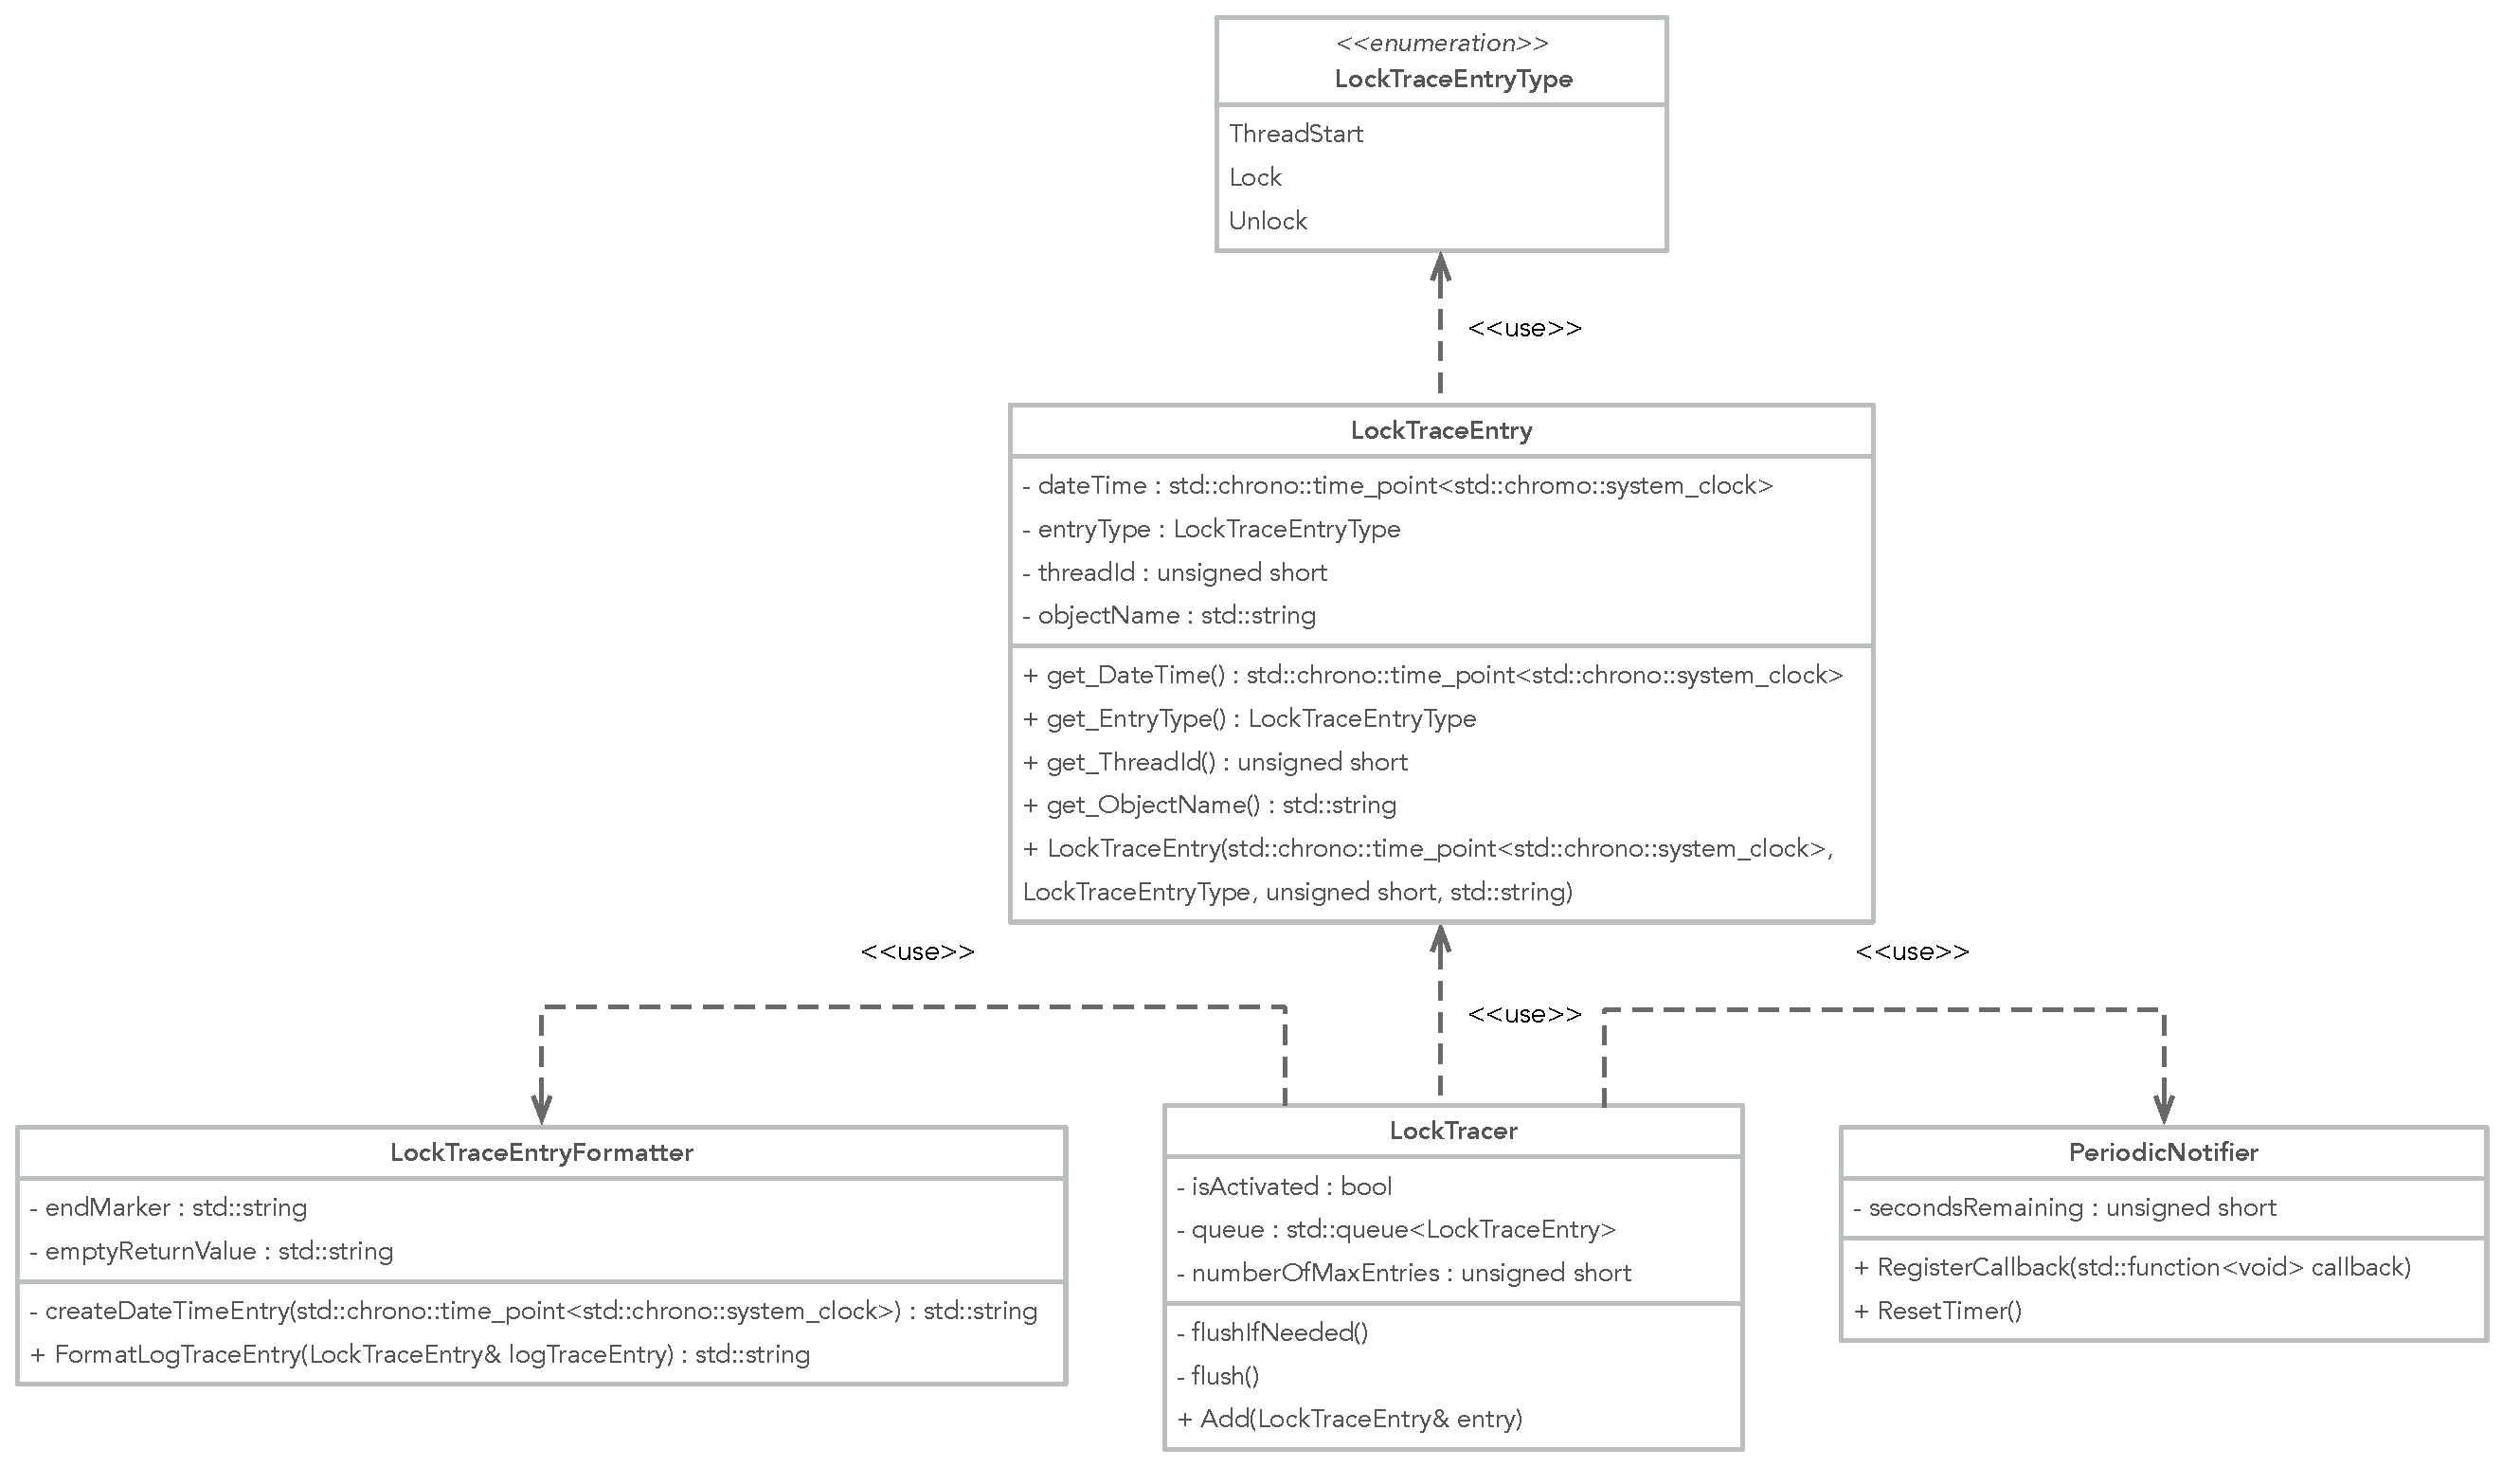
\includegraphics[width=\linewidth]{LockTrace_Design.eps}
  \caption{UML Klassendiagramm für Trace-Funktionalität}
  \label{fig:LockTrace_Design}
\end{figure}

In \cref{fig:LockTrace_Design} sind die benötigten Klassen dargestellt. Die
notwendigen Informationen für einen Trace-Eintrag werden in der Klasse
\texttt{LockTraceEntry} gehalten. Für den Zeitunkt wird der Typ 
\texttt{chrono::time\_point} vom Typ \texttt{chrono::high\_resolution\_clock}
verwendet. Der Typ \texttt{chrono::high\_resolution\_clock} stellt einen
Zeitpunkt mit der höchstmöglichen Genauigkeit der jeweiligen Implementierung dar
{TODO: Referenz auf C++11}. Für die spätere Visualisierung ist eine hohe
Genauigkeit notwendig, um nahezu parallel aufgetretene Lock-Ereignisse
chronologisch getrennt visualisieren zu können. Die Klasse
\texttt{LockTraceEntryFormatter} erstellt mit der Methode
\texttt{FormatLogTraceEntry} aus einem \texttt{LockTraceEntry} eine
Zeichenkette, welche einer Zeile in der Trace-Datei entspricht. Diese Klasse
wird als Singleton implementiert, da zur Laufzeit immer nur genau eine Instanz
benötigt wird. Die Klasse \texttt{LockTracer} stellt die Methode \texttt{Add}
zur Verfügung, welche von der OpenPEARL Laufzeitumgebung aufgerufen wird. Mit
Hilfe der Methode können Lock-Ereignisse erstellt werden. Die Methode
\texttt{IsEnabled} gibt den aktuellen Zustand der \texttt{LockTracer} Instanz
zurück. Mithilfe dieser Methode kann ein Aufrufer prüfen, ob die
Trace-Funktionalität aktiviert ist. Ist dies nicht der Fall, muss die
\texttt{Add} Methode nicht aufgerufen und somit auch kein
\texttt{LockTraceEntry} Objekt erzeugt werden. Die Klasse wird ebenfalls als
Singleton implementiert, damit nur eine Instanz zur Laufzeit verwendet werden
kann. Das Speichern der Ereignisse in die Trace-Datei ist kostspielig und soll
daher nicht für jeden Eintrag gemacht werden. Die Klasse \texttt{LockTracer}
reiht dazu die einzelnen Lock-Ereignisse, welche über die \texttt{Add} Methode
hinzugefügt werden, in eine Warteschlange ein. Sobald eine spezifizierte Anzahl
erreicht ist, wird die Warteschlange geleert und in die Trace-Datei geschrieben.
Die Anzahl kann über die Umgebungsvariable
\texttt{OpenPEARL\_LockTracer\_MaxEntries} spezifiziert werden. Die
Umgebungsvariable wird bei der Initialisierung der \texttt{LockTracer}
Implementierung ausgelesen und in der Variable \texttt{numberOfMaxEntries}
gespeichert. Das Hinzufügen der Ereignisse in die Warteschlange kann parallel
erfolgen und muss daher Thread sicher implementiert werden. Eine Möglichkeit
wäre, die einzelnen Zugriffe über einen Lock zu synchronisieren. Dies würde die
Laufzeit der Anwendung stark negativ beeinflussen. Deswegen wird eine lock freie
Implementierung einer Warteschlange verwendet
\autocite{Moody_Camels_Concurrentqueue}. Die Warteschlange garantiert eine
Thread sichere Implementierung, aber keine Sortierung innerhalb der
Warteschlange. Es kann passieren, dass Lock-Ereignisse in einer anderen
Reihenfolge aus der Warteschlange herausgenommen werden als sie eingefügt
wurden. Beim Auslesen der Trace-Datei muss daher anfangs eine Sortierung der
Einträge gemäß ihres Zeitpunkts durchgeführt werden. Der Dateipfad zur
Speicherung der Trace-Datei wird über die Umgebungsvariable
\texttt{OpenPEARL\_LockTracer\_Path} definiert und bei der Initialisierung der
\texttt{LockTracer} Implementierung in der Variable \texttt{filePath}
gespeichert. Die dritte Umgebungsvariable
\texttt{OpenPEARL\_LockTracer\_Enabled} wird zur Aktivierung der
Trace-Funktionalität verwendet. Wenn die Umgebungsvariable gesetzt ist und den
Wert \texttt{true} hat, wird die Trace-Funktionalität aktiviert. Ansonsten
werden alle Aufrufe zur \texttt{Add} Methode direkt über eine \texttt{return}
Anweisung beendet. Dadurch wird die Laufzeit der Anwendung bei deaktivierter
Trace-Funktionalität nicht beeinflusst.

In der OpenPEARL Laufzeitumgebung werden die \textit{REQUEST} und
\textit{RELEASE} Anweisungen in der Semaphore Implementierung unter
runtime/common/Semaphore.cc implementiert. Bei einer Erhöhung oder einer
Verringerung eines Semaphors muss ein Logeintrag erzeugt werden. Bei einer
Erhöhung muss der \texttt{LockTraceEntryType} \texttt{Unlock} bei einer
Verringerung der \texttt{LockTraceEntryType} \texttt{Lock} verwendet werden. Die
Klassen für die Implementierung des LockTracers müssen bei der Kompilierung der
OpenPEARL Laufzeitumgebung mit einbezogen werden. In der Datei
runtime/common/Files.common sind alle Dateien aufgeführt, welche bei der
Kompilierung einbezogen werden. Dort müssen die Dateien, die aus
\cref{fig:LockTrace_Design} entstehen eingetragen werden.

\section{Analysieren der Trace-Datei}
\label{section:Analysieren der Trace-Datei}
Als Eingabe dient die in \cref{section:Erzeugung der Trace-Datei} erzeugte
Trace-Datei. Die chronologische Darstellung wird, wie in
\cref{fig:Timeline_Example} skizziert, über einen zwei dimensionalen Graphen
realisiert. Die Ordinate bildet die Zeit ab, wobei nur das Delta in
Mikrosekunden zwischen den einzelnen Ereignissen dargestellt wird. Für jeden
Thread wird ein Eintrag auf der Abszisse gemacht. Es wird zwischen zwei
Ereignissen unterschieden. Wird ein \texttt{SEMA} Objekt in Besitz genommen,
wird ein roter, für das Freigeben eines \texttt{SEMA} Objekts ein grüner, Kreis
gezeichnet. Die Beschriftung eines Kreises enthält den Namen des \texttt{SEMA}
Objekts.

\begin{figure}[ht]
  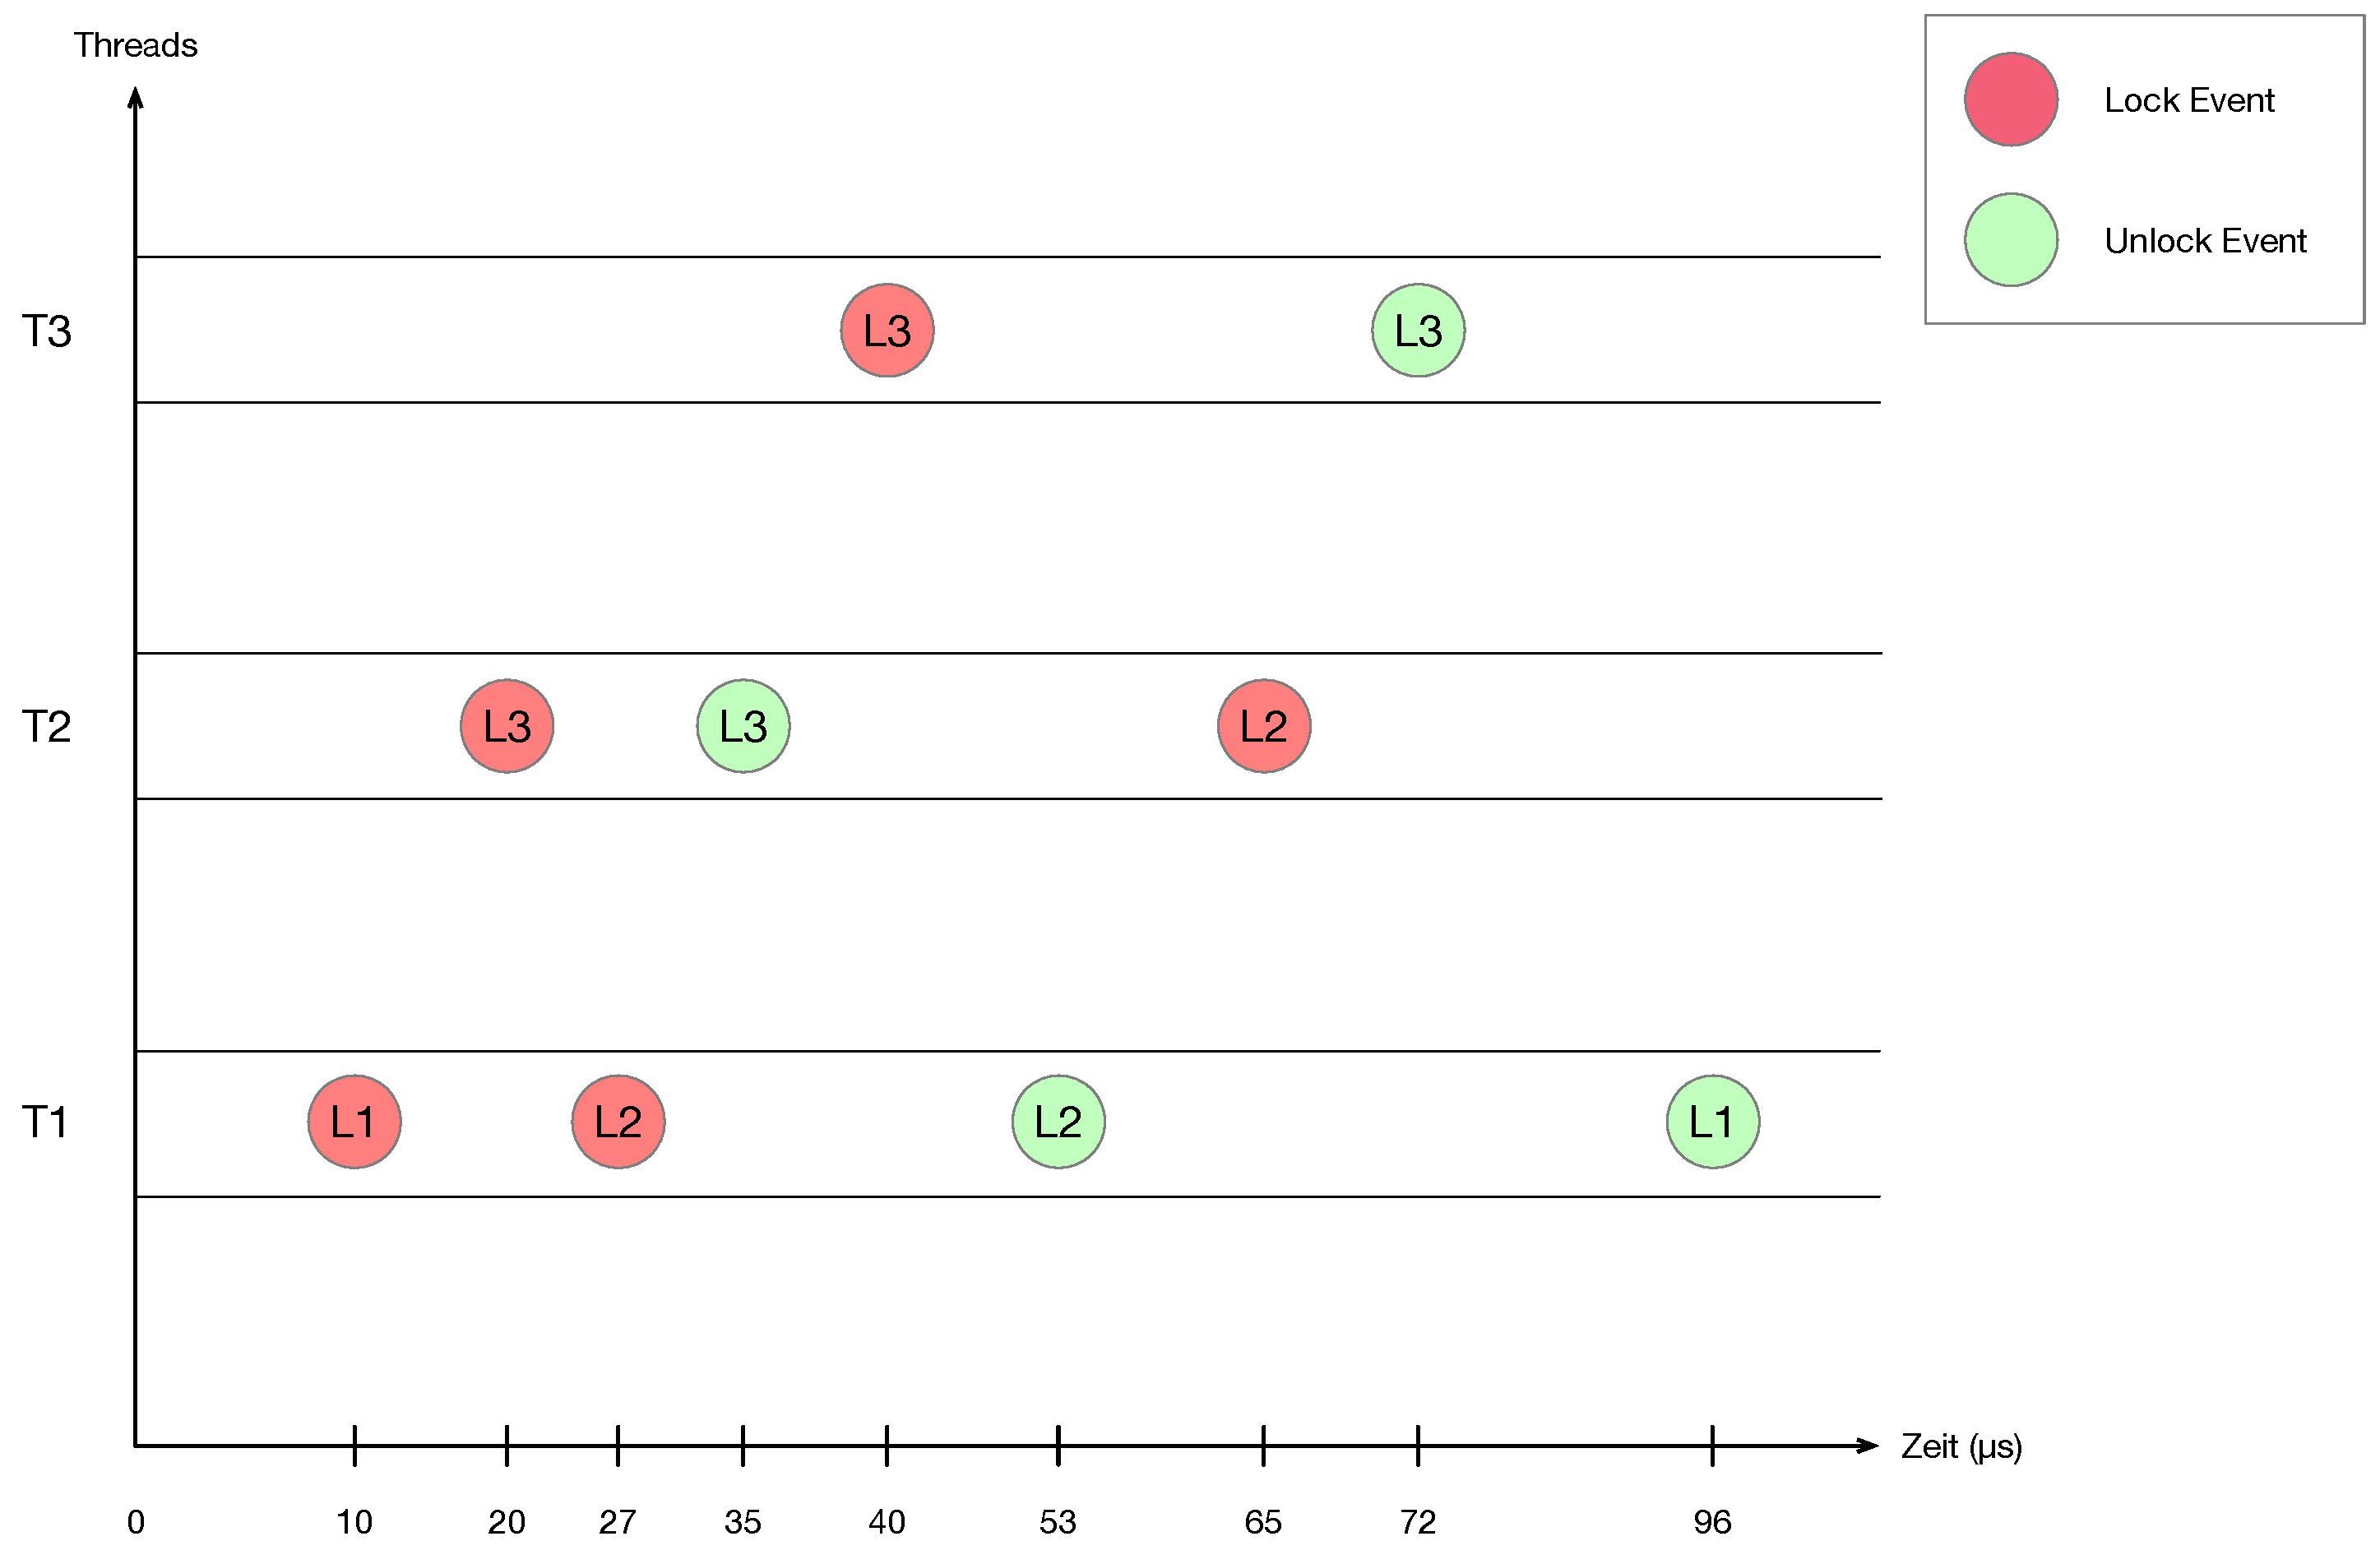
\includegraphics[width=\linewidth]{Timeline_Example.eps}
  \caption{Visualisierung der chronologischen Verwendung von \textit{SEMA} Objekten}
  \label{fig:Timeline_Example}
\end{figure}

\section{Erweiterung: Potenzielle Deadlocks}
\label{section:Erweiterung: Potenzielle Deadlocks}
Der in \cref{section:MagicLock} beschrieben Algorithmus wird dazu verwendet, um
potentielle Deadlocks in der aus \cref{section:Erzeugung der Trace-Datei}
erstellten Trace-Datei zu finden. 

\begin{figure}[ht]
  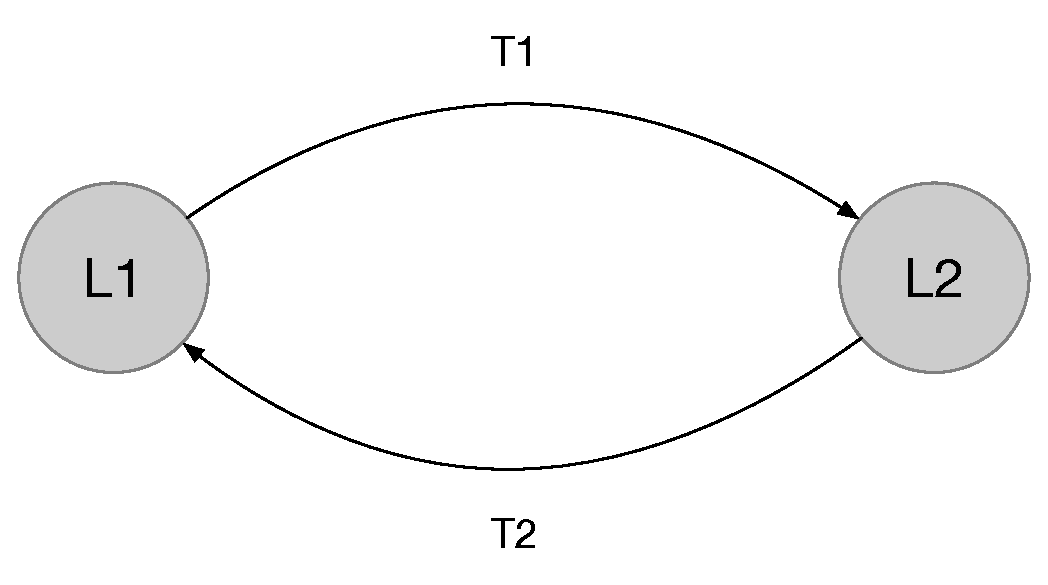
\includegraphics[width=\linewidth/2]{Magiclock_Example.eps}
  \caption{Beispielhafte Visualisierung eines potentiellen Deadlocks}
  \label{fig:Magiclock_Example}
\end{figure}

Potentielle Deadlocks werden wie in \cref{fig:Magiclock_Example} skizziert als
gerichteter Graph dargestellt. Knoten repräsentieren Lockobjekte, Kanten
repräsentieren die Inbesitznahme eines Lockobjekts und die Beschriftung an einer
Kante bezeichnet den ausführenden Thread. In dem skizzierten Beispiel ist ein
potentieller Deadlock zwischen den Threads \textit{T1} und \textit{T2}
dargestellt. Der Thread \textit{T1} nimmt das Lockobjekt \textit{L2} in Besitz
während dieser bereits \textit{L1} besitzt. Dies ist zu erkennen an der Kante
vom Knoten \textit{L1} zum Knoten \textit{L2} mit der Bezeichnung \textit{T1}.
Der Thread \textit{T2} nimmt in dem Beispiel das Lockobjekt \textit{L1} in
Besitz während dieser bereits \textit{L2} besitzt. Dies kann zu einem Deadlock
führen, wenn \textit{T1} das Lockobjekt \textit{L1} und \textit{T2} das
Lockobjekt \textit{L2} gleichzeitig besitzen.
\stopcontents

\startcontents
\chapter{Implementierung}
\thispagestyle{fancy}
\printcontents{l}{1}{\setcounter{tocdepth}{5}}
\section{Trace Funktion}
\label{section:Implementierung:Trace Funktion}
\begin{itemize}
  \item Vorstellung der Implementierung der Trace Funktionalität in PEARL
\end{itemize}

\section{Analyse Programm}
\label{section:Implementierung:Analyse Programm}
\begin{itemize}
  \item Vorstellung der Implementierung des Analyse Programms in Java
  \item Grafiken/Screenshots mit Analyse Beispielen
\end{itemize}

\section{Visualisierung von potenziellen Deadlocks}
\label{section:Implementierung:Visualisierung von potenziellen Deadlocks}
\begin{itemize}
  \item Vorstellung der Implementierung des Algorithmus zur Erkennung von
  potenziellen Deadlocks
  MagicLock klassifiziert dazu jedes Lock-Objekt in eine der folgenden Mengen:
  \begin{enumerate}
    \item \textbf{Independent-set} = $\{m \mid m \in Locks, indegree(m) = 0 \land outdegree(m) = 0\}$
    \item \textbf{Intermediate-set} = $\{m \mid m \in Locks, (indegree(m) = 0 \lor outdegree(m) = 0) \land \lnot (indegree(m) = 0 \land outdegree(m) = 0)\}$
    \item \textbf{Inner-set} = $\{m \mid m \in Locks, (\exists (t,m,L) \in D, \forall n \in L, n \in \text{Intermediate-set} \cup \text{Inner-set}) \lor (\exists (t,n,L) \in D, m \in L \land n \in \text{Intermediate-set} \cup \text{Inner-set})\}$
    \item \textbf{Cyclic-set} = $\{m \mid m \in Locks, m \notin \text{Independent-set} \cup \text{Intermediate-set} \cup \text{Inner-set}\}$
  \end{enumerate}
  \item Grafiken/Screenshots mit Analyse Beispielen
\end{itemize}
\stopcontents

\startcontents
\chapter{Validierung}
\thispagestyle{fancy}
\printcontents{l}{1}{\setcounter{tocdepth}{5}}
\section{Trace Funktion}\label{Validierung:Trace Funktion}
\label{section:ValidierungTraceFunktion}
Um die Trace-Funktionalität in OpenPEARL zu prüfen werden folgende
Umgebungsvariablen verwendet:
\begin{itemize}
  \item \emph{OpenPEARL\-\_LockTracer\-\_Enabled} = false
  \item \emph{OpenPEARL\-\_LockTracer\-\_Path} = /tmp/LockTracer/
  \item \emph{OpenPEARL\-\_LockTracer\-\_MaxEntries} = 1
\end{itemize}
Zum Testen wird die OpenPEARL Anwendung aus \cref{lst:OpenPEARLTraceTest}
verwendet. 
\begin{listing}[ht]
  \inputminted[frame=lines,linenos]{vim}{./OpenPEARL/TraceTest.prl}
  \caption{OpenPEARL Anwendung zum Testen der Trace-Funktionalität}
  \label{lst:OpenPEARLTraceTest}
\end{listing}
Es wird ein Thread \texttt{T1} erzeugt, welcher die \emph{SEMA} Variable
\texttt{test\_sema} insgesamt neun Mal freigibt und in Besitz nimmt. Wird die
Anwendung ausgeführt wird keine Trace-Datei angelegt. Wird die Umgebungsvariable
\emph{OpenPEARL\-\_LockTracer\-\_Enabled} auf \texttt{true} gesetzt, wird die
Trace-Datei aus \cref{lst:OpenPEARLTraceResult} erzeugt.
\begin{listing}[ht]
  \begin{minipage}[ht]{\linewidth}
    \begin{multicols}{2}
      \inputminted[linenos]{text}{./OpenPEARL/TraceTestResult.log}
    \end{multicols}
    \caption{Trace-Datei die bei aktivierter Trace-Funktionalität aus \cref{lst:OpenPEARLTraceTest} erzeugt wird}
  \label{lst:OpenPEARLTraceResult}
  \end{minipage}
\end{listing}

Die Tests zur Messung der Laufzeit und der Speicherauslastung werden in einer
virtuellen Maschine mit Debian 9 Betriebssystem, 4 CPU Kernen und 2~GB
Arbeitsspeicher durchgeführt. Das Host System läuft mit dem Betriebssystem macOS
10.15.4 und verfügt über einen Intel Core i7 mit 3,1 GHz, 16~GB Arbeitsspeicher
und einer 512~GB PCIe SSD. Zur Messung der Laufzeit wird das Pythonskipt aus
\cref{lst:Python_Benchmark_CPU} und zur Messung der Speicherauslastung das
Pythonskipt aus \cref{lst:Python_Benchmark_Memory} verwendet.
\begin{listing}[ht]
  \inputminted[frame=lines,linenos]{python}{./Python/benchmark_cpu.py}
  \caption{Pythonskipt zur Messung der Laufzeit}
  \label{lst:Python_Benchmark_CPU}
\end{listing} 
\begin{listing}[ht]
  \inputminted[frame=lines,linenos]{python}{./Python/benchmark_memory.py}
  \caption{Pythonskipt zur Messung der Speicherauslastung}
  \label{lst:Python_Benchmark_Memory}
\end{listing}
Für die Tests wird eine OpenPEARL Anwendung verwendet, welche zehn Threads
erzeugt, die jeweils nacheinander zwei \emph{SEMA} Objekte in Besitz nehmen und
wieder freigeben. Dabei verwendet der Thread \emph{T1} die Objekte
\emph{L01} und \emph{L02}, der Thread \emph{T2} die Objekte \emph{L02}
und \emph{L03}, bis zum letzten Thread \emph{T10}, welcher die Objekte
\emph{L10} und \emph{L01} verwendet. Ingesamt werden 400.000 Einträge erzeugt.
Das Ergebnis der Laufzeitmessung ist in \cref{fig:BenchmarkCpuResults}
dargestellt. 
\begin{figure}[ht]
  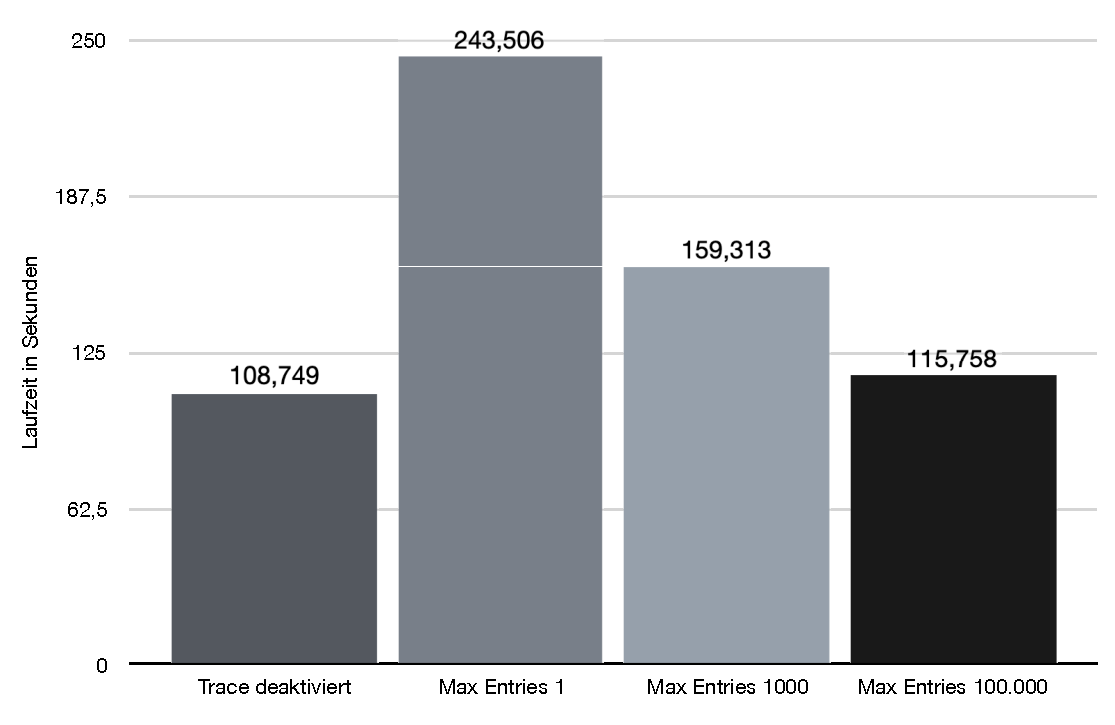
\includegraphics[width=\linewidth]{Benchmark_CPU_Results.eps}
  \footnotesize\sffamily\textbf{Quelle:} Eigene Darstellung
  \caption{Ergebnisse der Laufzeitmessung der Trace-Funktionalität in OpenPEARL}
  \label{fig:BenchmarkCpuResults}
\end{figure}
Eine höhere Anzahl an gepufferten Objekten führt bis zu einem bestimmten Punkt
zu einer besseren Laufzeit. Bei einer Puffergröße von 100.000 gibt es nur noch
einen sehr geringen Unterschied zwischen aktivierter und deaktivierter
Trace-Funktionalität. Wird die Puffergröße auf 500.000 gesetzt, passen alle
Einträge in den Puffer und werden beim Beenden der Anwendung in die Trace-Datei
geschrieben. Die Laufzeit verbessert sich bei dieser Größe jedoch nicht weiter,
sondern verschlechtert sich leicht. Bereits der Unterschied zwischen den
Puffergrößen 1.000 und 100.000 zeigt, dass die Puffergröße nicht beliebig hoch
gesetzt werden sollte, um eine optimale Laufzeit zu erhalten. Die Puffergröße
muss individuell für das Zielsystem ermittelt werden. Das Ergebnis der Messung
der Speicherauslastung ist in \cref{fig:BenchmarkMemoryResults} dargestellt.
\begin{figure}[ht]
  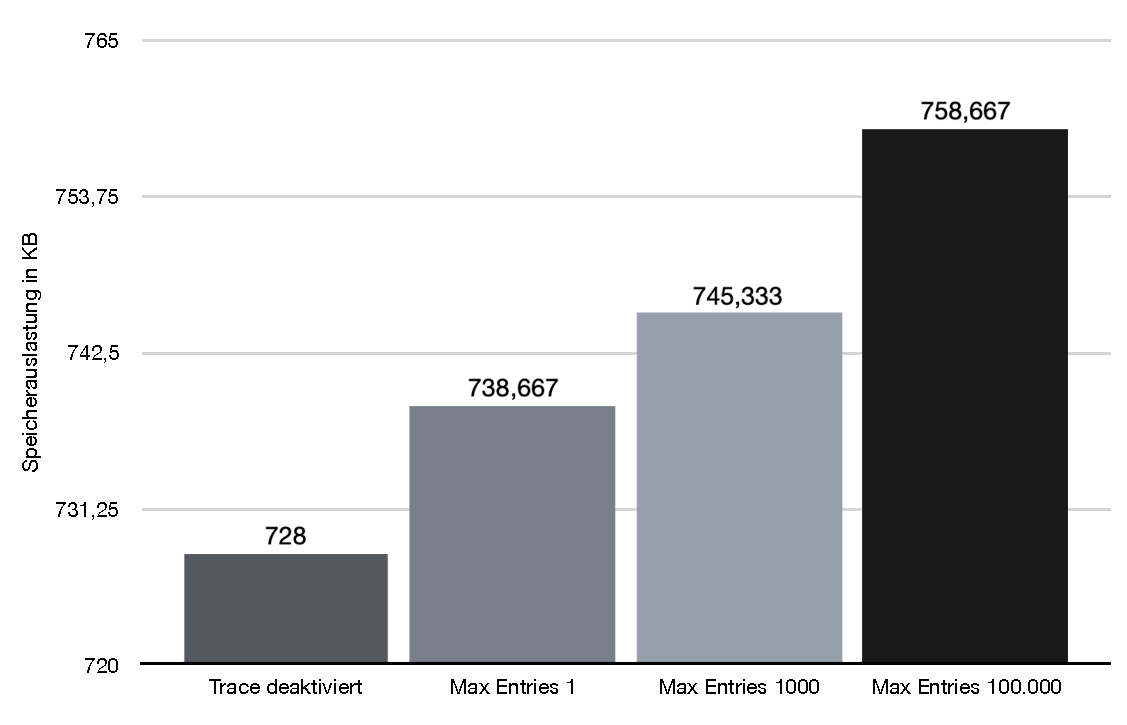
\includegraphics[width=\linewidth]{Benchmark_Memory_Results.eps}
  \footnotesize\sffamily\textbf{Quelle:} Eigene Darstellung
  \caption{Ergebnisse der Speicherauslastung der Trace-Funktionalität in OpenPEARL}
  \label{fig:BenchmarkMemoryResults}
\end{figure}
Je größer der verwendete Puffer ist, desto höher ist auch die
Speicherauslastung. Für das verwendete Testsystem ist eine Puffergröße von 1.000
ein guter Kompromiss zwischen Laufzeit und Speicherauslastung. Ist die Laufzeit
wichtiger und die Speicherauslastung kein Problem, sollte eine Puffergröße von
100.000 gewählt werden.

\section{Analyse Programm}
\label{section:ValidierungAnalyseProgramm}
Für die chronologische Darstellung der Lockobjekte wird die Trace-Datei aus
\cref{lst:ExampleTraceFile} mit drei Threads und neun Lockobjekten verwendet.
\begin{listing}[ht]
  \begin{minipage}[ht]{\linewidth}
    \begin{multicols}{3}
      \inputminted[linenos]{text}{./Examples/ExampleTraceFile.log}
    \end{multicols}
    \caption{Beispielhafte Trace-Datei mit einem potenziellen Deadlock}
    \label{lst:ExampleTraceFile}
  \end{minipage}
\end{listing}
In dem Beispiel gibt es zusätzlich zwei Einträge mit dem gleichen Zeitstempel in
den Zeilen 3 und 4 sowie in den Zeilen 13 und 14. Die Ausgabe der Anwendung aus
\cref{section:Implementierung:Analyse Programm} ist in
\cref{fig:LockTraceVisualization} dargestellt.
\begin{figure}[ht]
  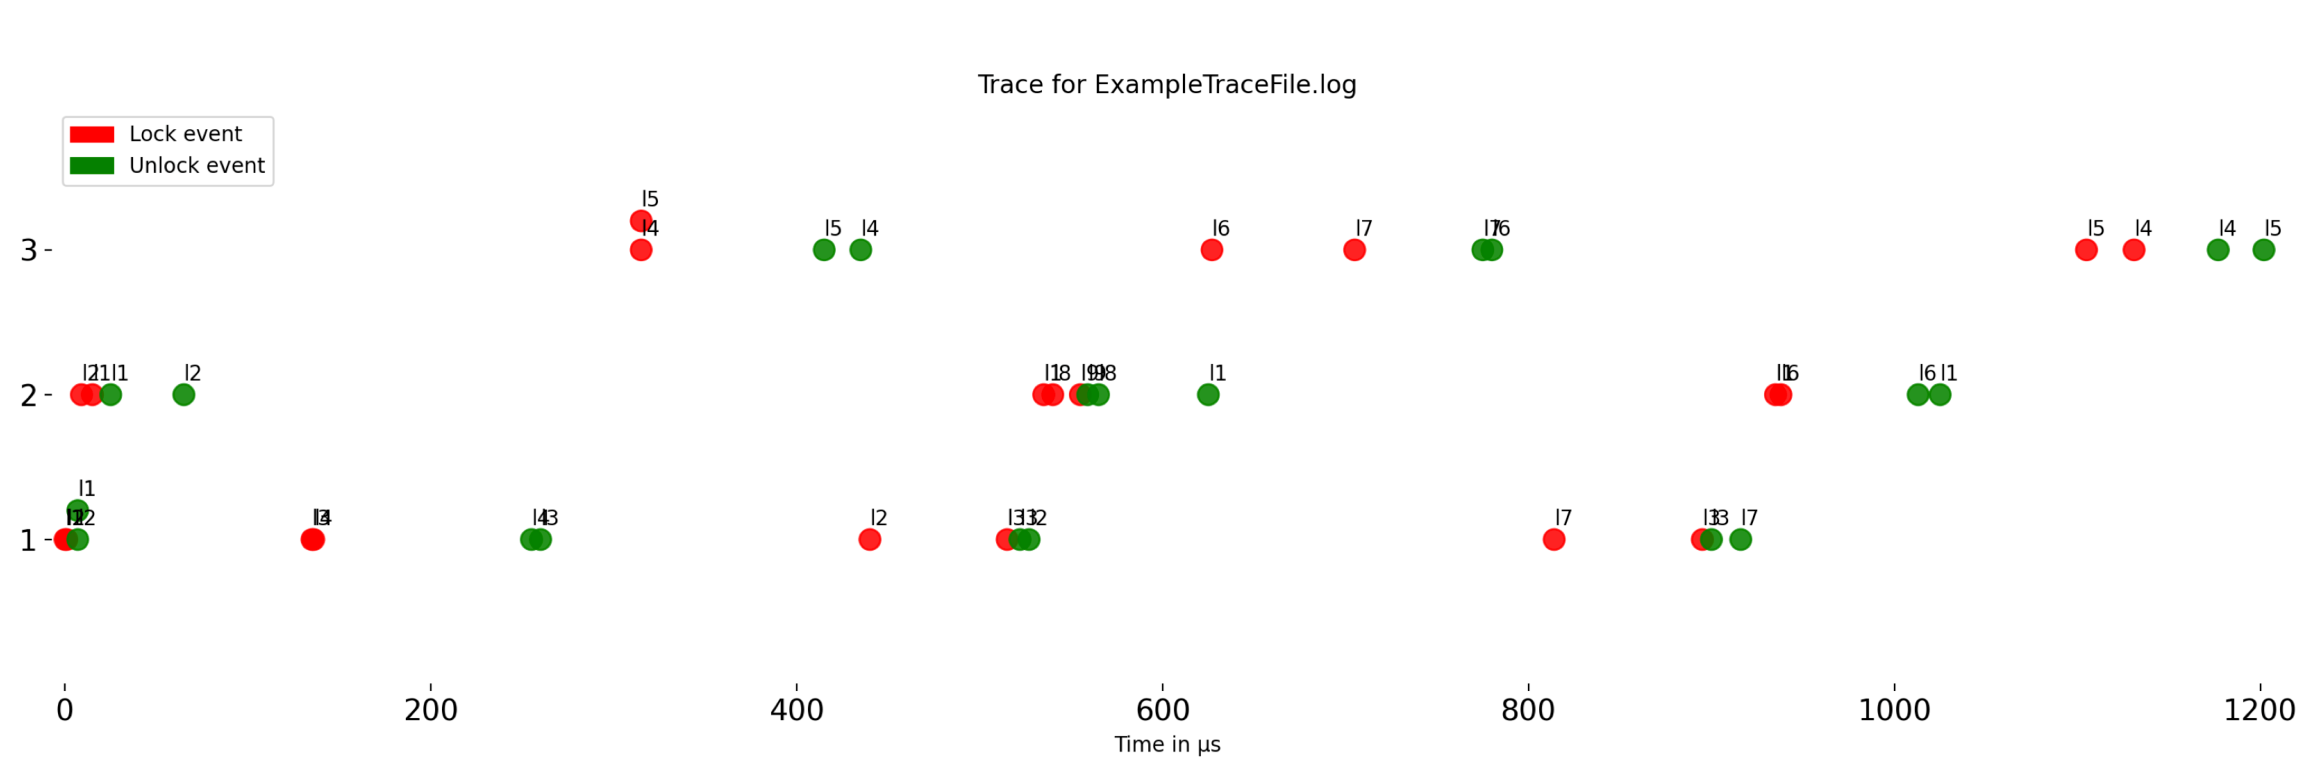
\includegraphics[width=\linewidth]{ExampleTraceFile.eps}
  \footnotesize\sffamily\textbf{Quelle:} Eigene Darstellung
  \caption{Ausgabe der Analyse-Anwendung}
  \label{fig:LockTraceVisualization}
\end{figure}

Die überlappenden Logeinträge können auseinander gezogen werden in dem in den
Graphen hineingezoomt wird. Die Vergrößerung auf 70 Mikrosekunden ist in
\cref{fig:LockTraceVisualizationZoomed} dargestellt.
\begin{figure}[ht]
  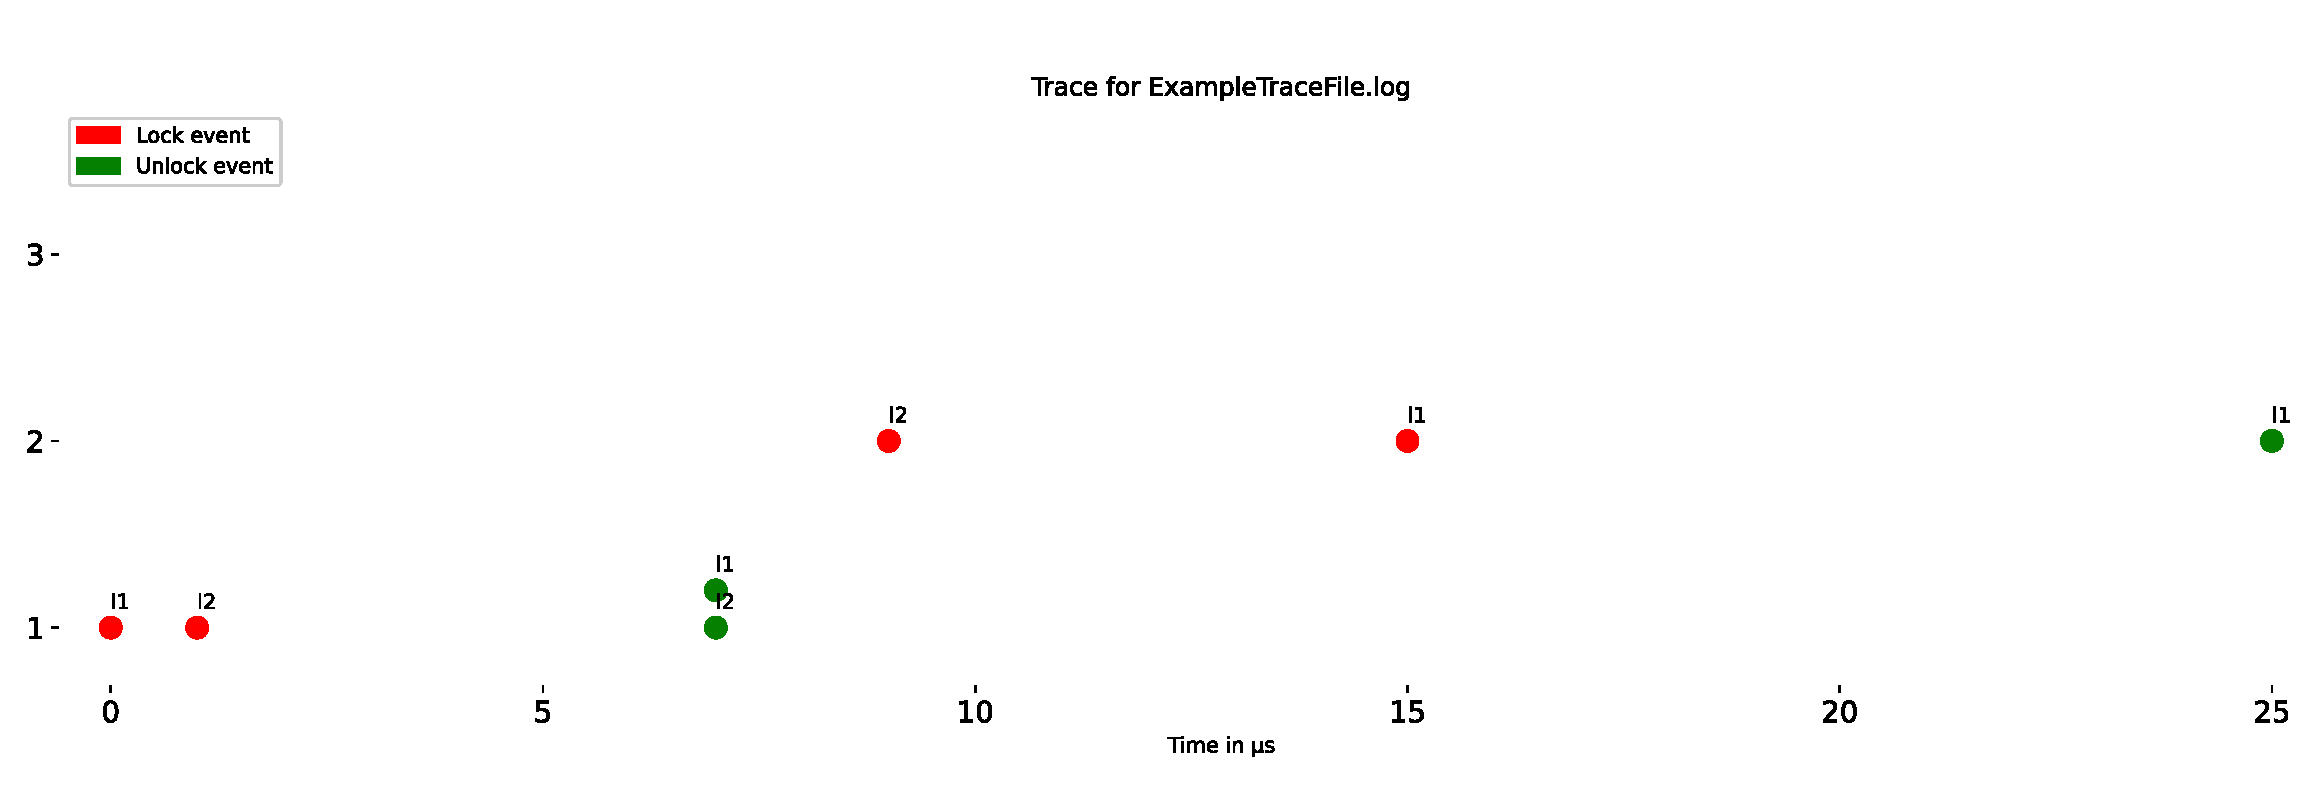
\includegraphics[width=\linewidth]{ExampleTraceFileZoomed.eps}
  \footnotesize\sffamily\textbf{Quelle:} Eigene Darstellung
  \caption{Vergrößerte Darstellung von \cref{fig:LockTraceVisualization}}
  \label{fig:LockTraceVisualizationZoomed}
\end{figure}

Die einzelnen Logeinträge sind sichtbar und können auseinander gehalten werden.
Eine Überlappung wird trotz gleichen Zeitstempel verhindert, indem die
Logeinträge mit gleichen Zeitstempel bei sieben Mikrosekunden vertikal versetzt
dargestellt werden.

\section{Visualisierung von potenziellen Deadlocks}
\label{section:DeadlockVisualization}
Für die Visualisierung von potenziellen Deadlocks wird erneut die Trace-Datei
aus \cref{lst:ExampleTraceFile} verwendet. In dem Beispiel gibt es genau einen
potenziellen Deadlock zwischen den Threads \emph{1} und \emph{2}. In den Zeilen
1 und 2 nimmt der Thread \emph{1} die Lockobjekten \emph{l1} und \emph{l2}
nacheinander in Besitz. In den Zeilen 5 und 6 nimmt der Thread \emph{2} die
Lockobjekte \emph{l2} und \emph{l1} nacheinander in Besitz. Der potenzielle
Deadlock entsteht, da der Thread \emph{1} zuerst das Lockobjekt \emph{l1} in
Besitz nehmen kann und bevor dieser das Lockobjekt \emph{l2} in Besitz nehmen
kann, kann der Thread \emph{2} das Lockobjekt \emph{l2} bereits in seinen Besitz
genommen haben. Dadurch blockieren sich beide Threads gegenseitig und ein
Deadlock entsteht. Die Ausgabe der Anwendung zur Erkennung und Visualisierung
von potenziellen Deadlocks ist in \cref{fig:DeadlockVisualization} dargestellt.
\begin{figure}[ht]
  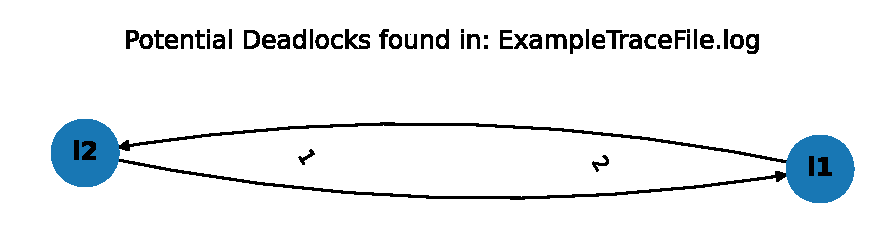
\includegraphics[width=\linewidth]{ExamplePotentialDeadlocks.eps}
  \footnotesize\sffamily\textbf{Quelle:} Eigene Darstellung
  \caption{Ergebnis der Erkennung von potenziellen Deadlocks aus \cref{lst:ExampleTraceFile}}
  \label{fig:DeadlockVisualization}
\end{figure}
Die Beschriftung der Kanten erfolgt immer zum Ende der Kante hin, zum Beispiel
gehört die Beschriftung \emph{1} zu der Kante von \emph{l1} zu \emph{l2}.
Zusätzlich zur grafischen Darstellung werden die Ergebnisse als
Zyklische-Lock-Dependency-Chain auf der Konsole ausgegeben. Für die verwendete
Trace-Datei wird "(1,l2,{l1}) (2,l1,{l2})" als potenzieller Deadlock auf der
Konsole ausgegeben.
\stopcontents

\startcontents
\chapter{Ausblick}
\thispagestyle{fancy}
\printcontents{l}{1}{\setcounter{tocdepth}{5}}
\section{Offene Punkte}
\begin{itemize}
  \item Aufzeigen was nicht gemacht wurde und warum (eventuell welche
  Synchronisationsmittel nicht erkannt werden)
\end{itemize}

\section{Weiterentwicklung}
\begin{itemize}
  \item Alle möglichen Synchronisationsmittel erkennen
  \item Trace Funktionalität in den OpenPEARL Compiler integrieren, so dass es
  mittels compiler flag an und ausgeschaltet werden kann
\end{itemize}
\stopcontents


\printbibliography

\end{document}